\appendix
\onecolumn
\clearpage

\section{LLM and Non-LLM Game Results}
\label{app:llm_nonllm}

This section presents the same equilibrium metrics for games involving both LLM and non-LLM agents. The comparison between these results and the LLM-only results reveals how the introduction of traditional game-theoretic strategies affects equilibrium behavior.

\begin{figure}[H]
\centering
\begin{tabular}{cc}
\multicolumn{2}{c}{\textbf{BG1 (\(\gamma=0.9\), \(R=3\))}} \\
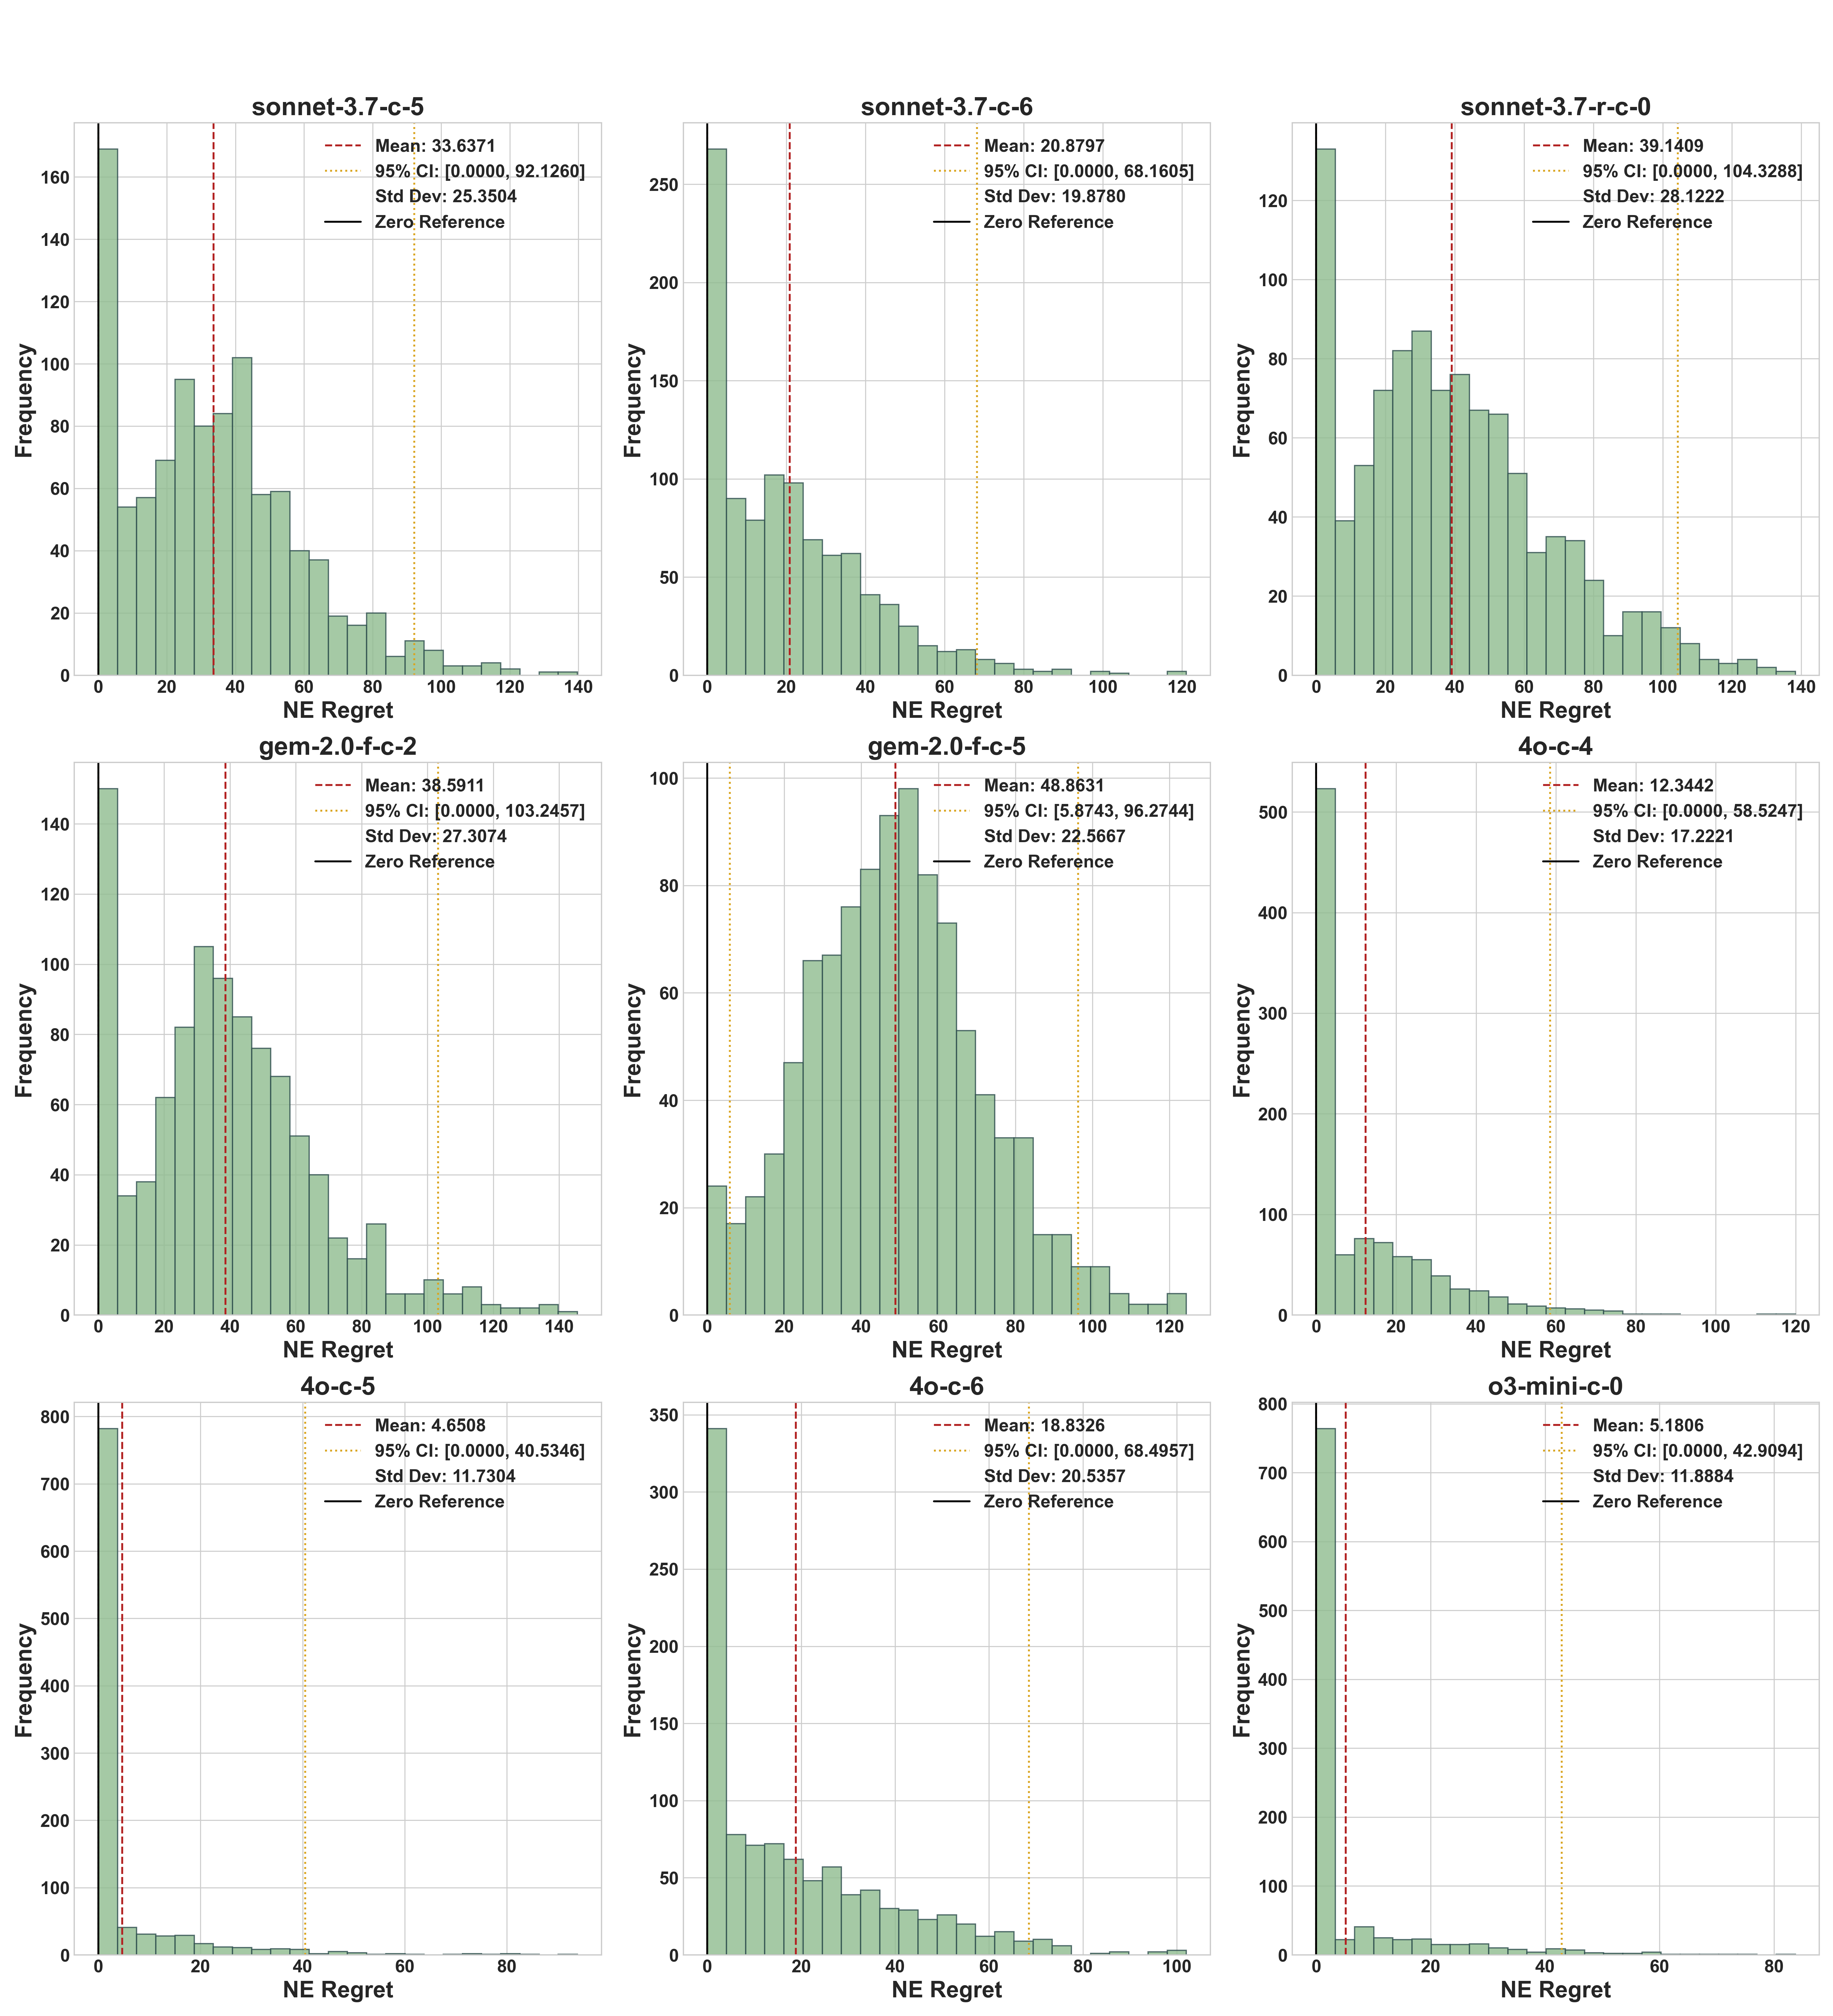
\includegraphics[width=0.46\textwidth]{icml_2025_workshop/bootstrap_distributions/llm_only/game_matrix_1/me_ne_regret.png} &
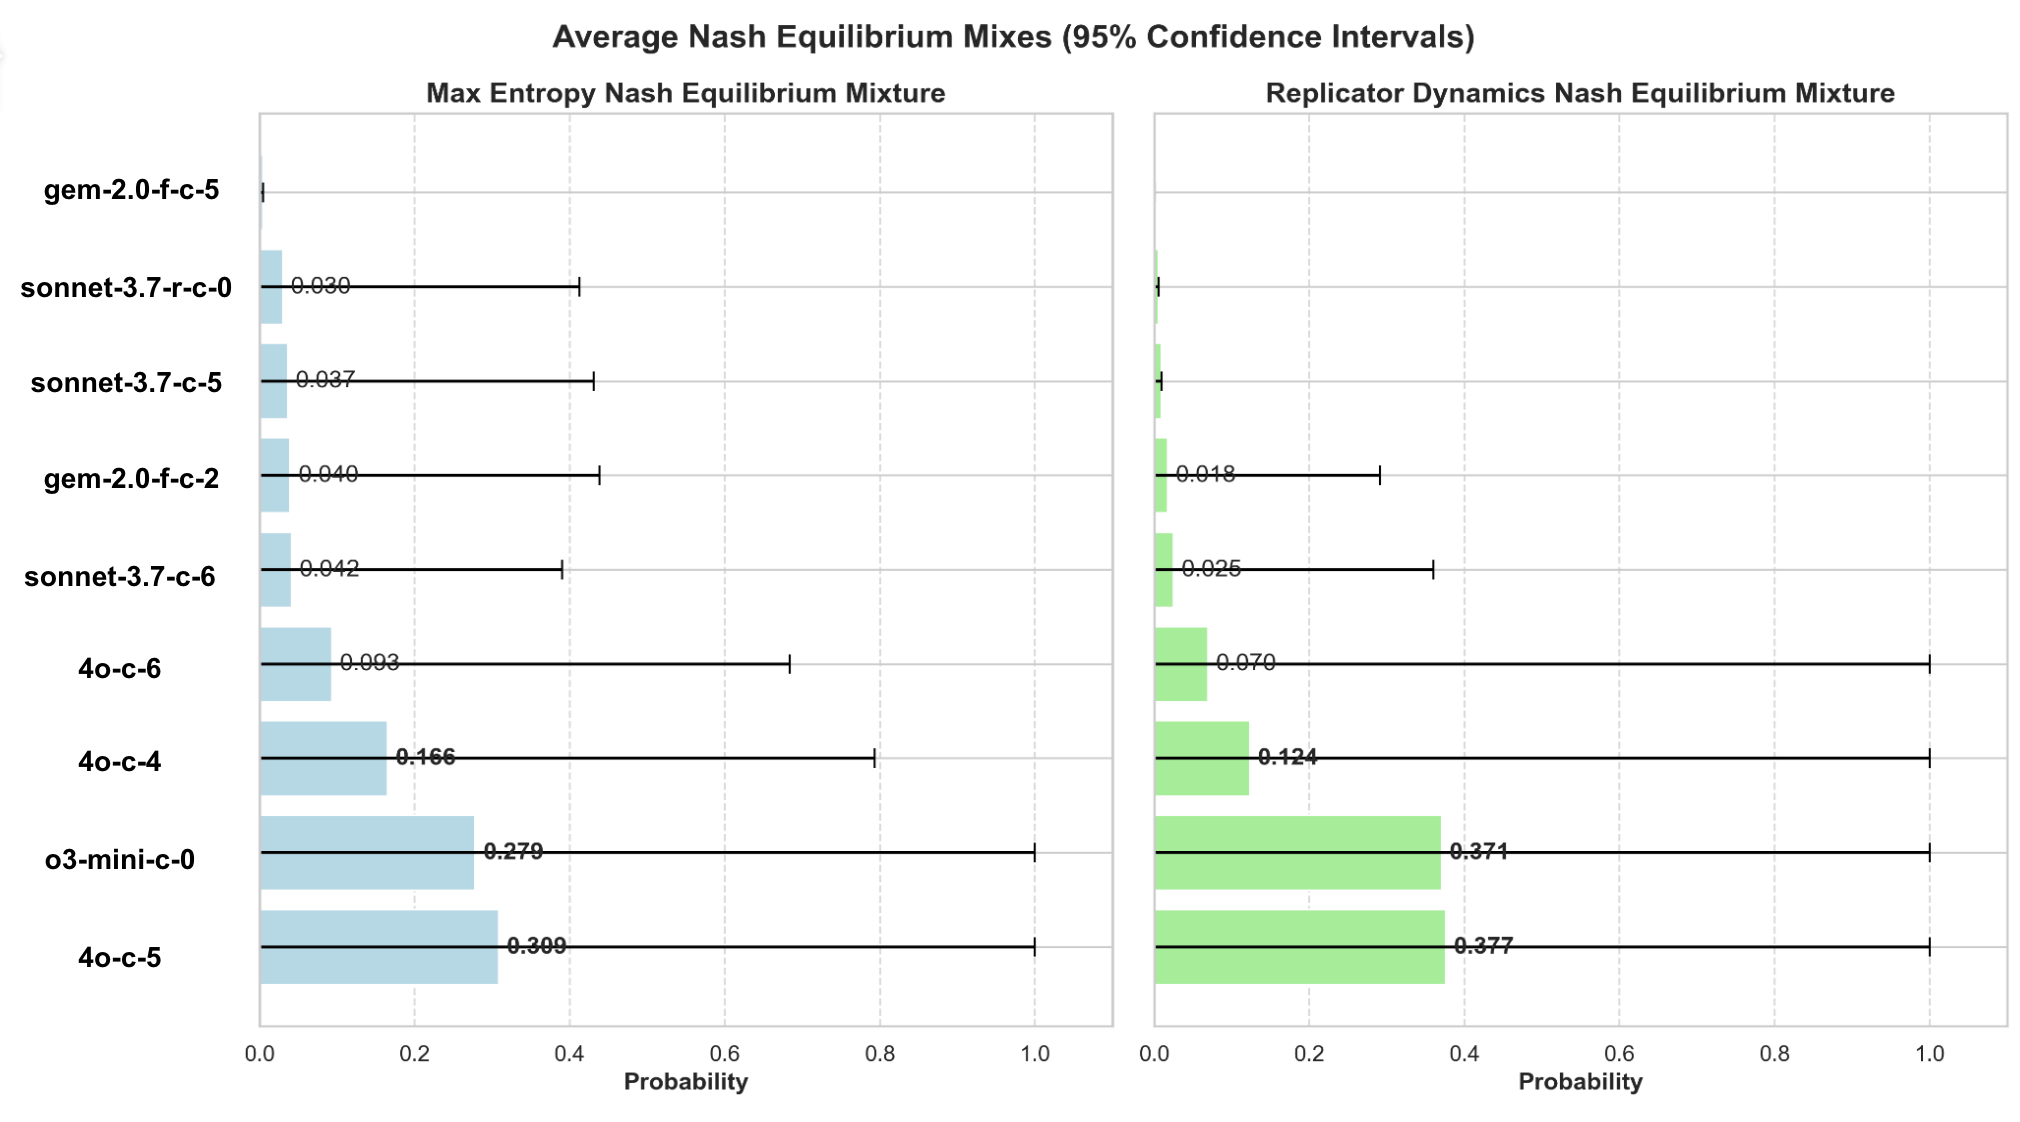
\includegraphics[width=0.46\textwidth]{icml_2025_workshop/bootstrap_distributions/llm_only/game_matrix_1/nash_mixture.png} \\
{\small ME-NE Regret} & {\small Nash Mixture} \\%[0.5cm]

\multicolumn{2}{c}{\textbf{BG2 (\(\gamma=0.98\), \(R=3\))}} \\
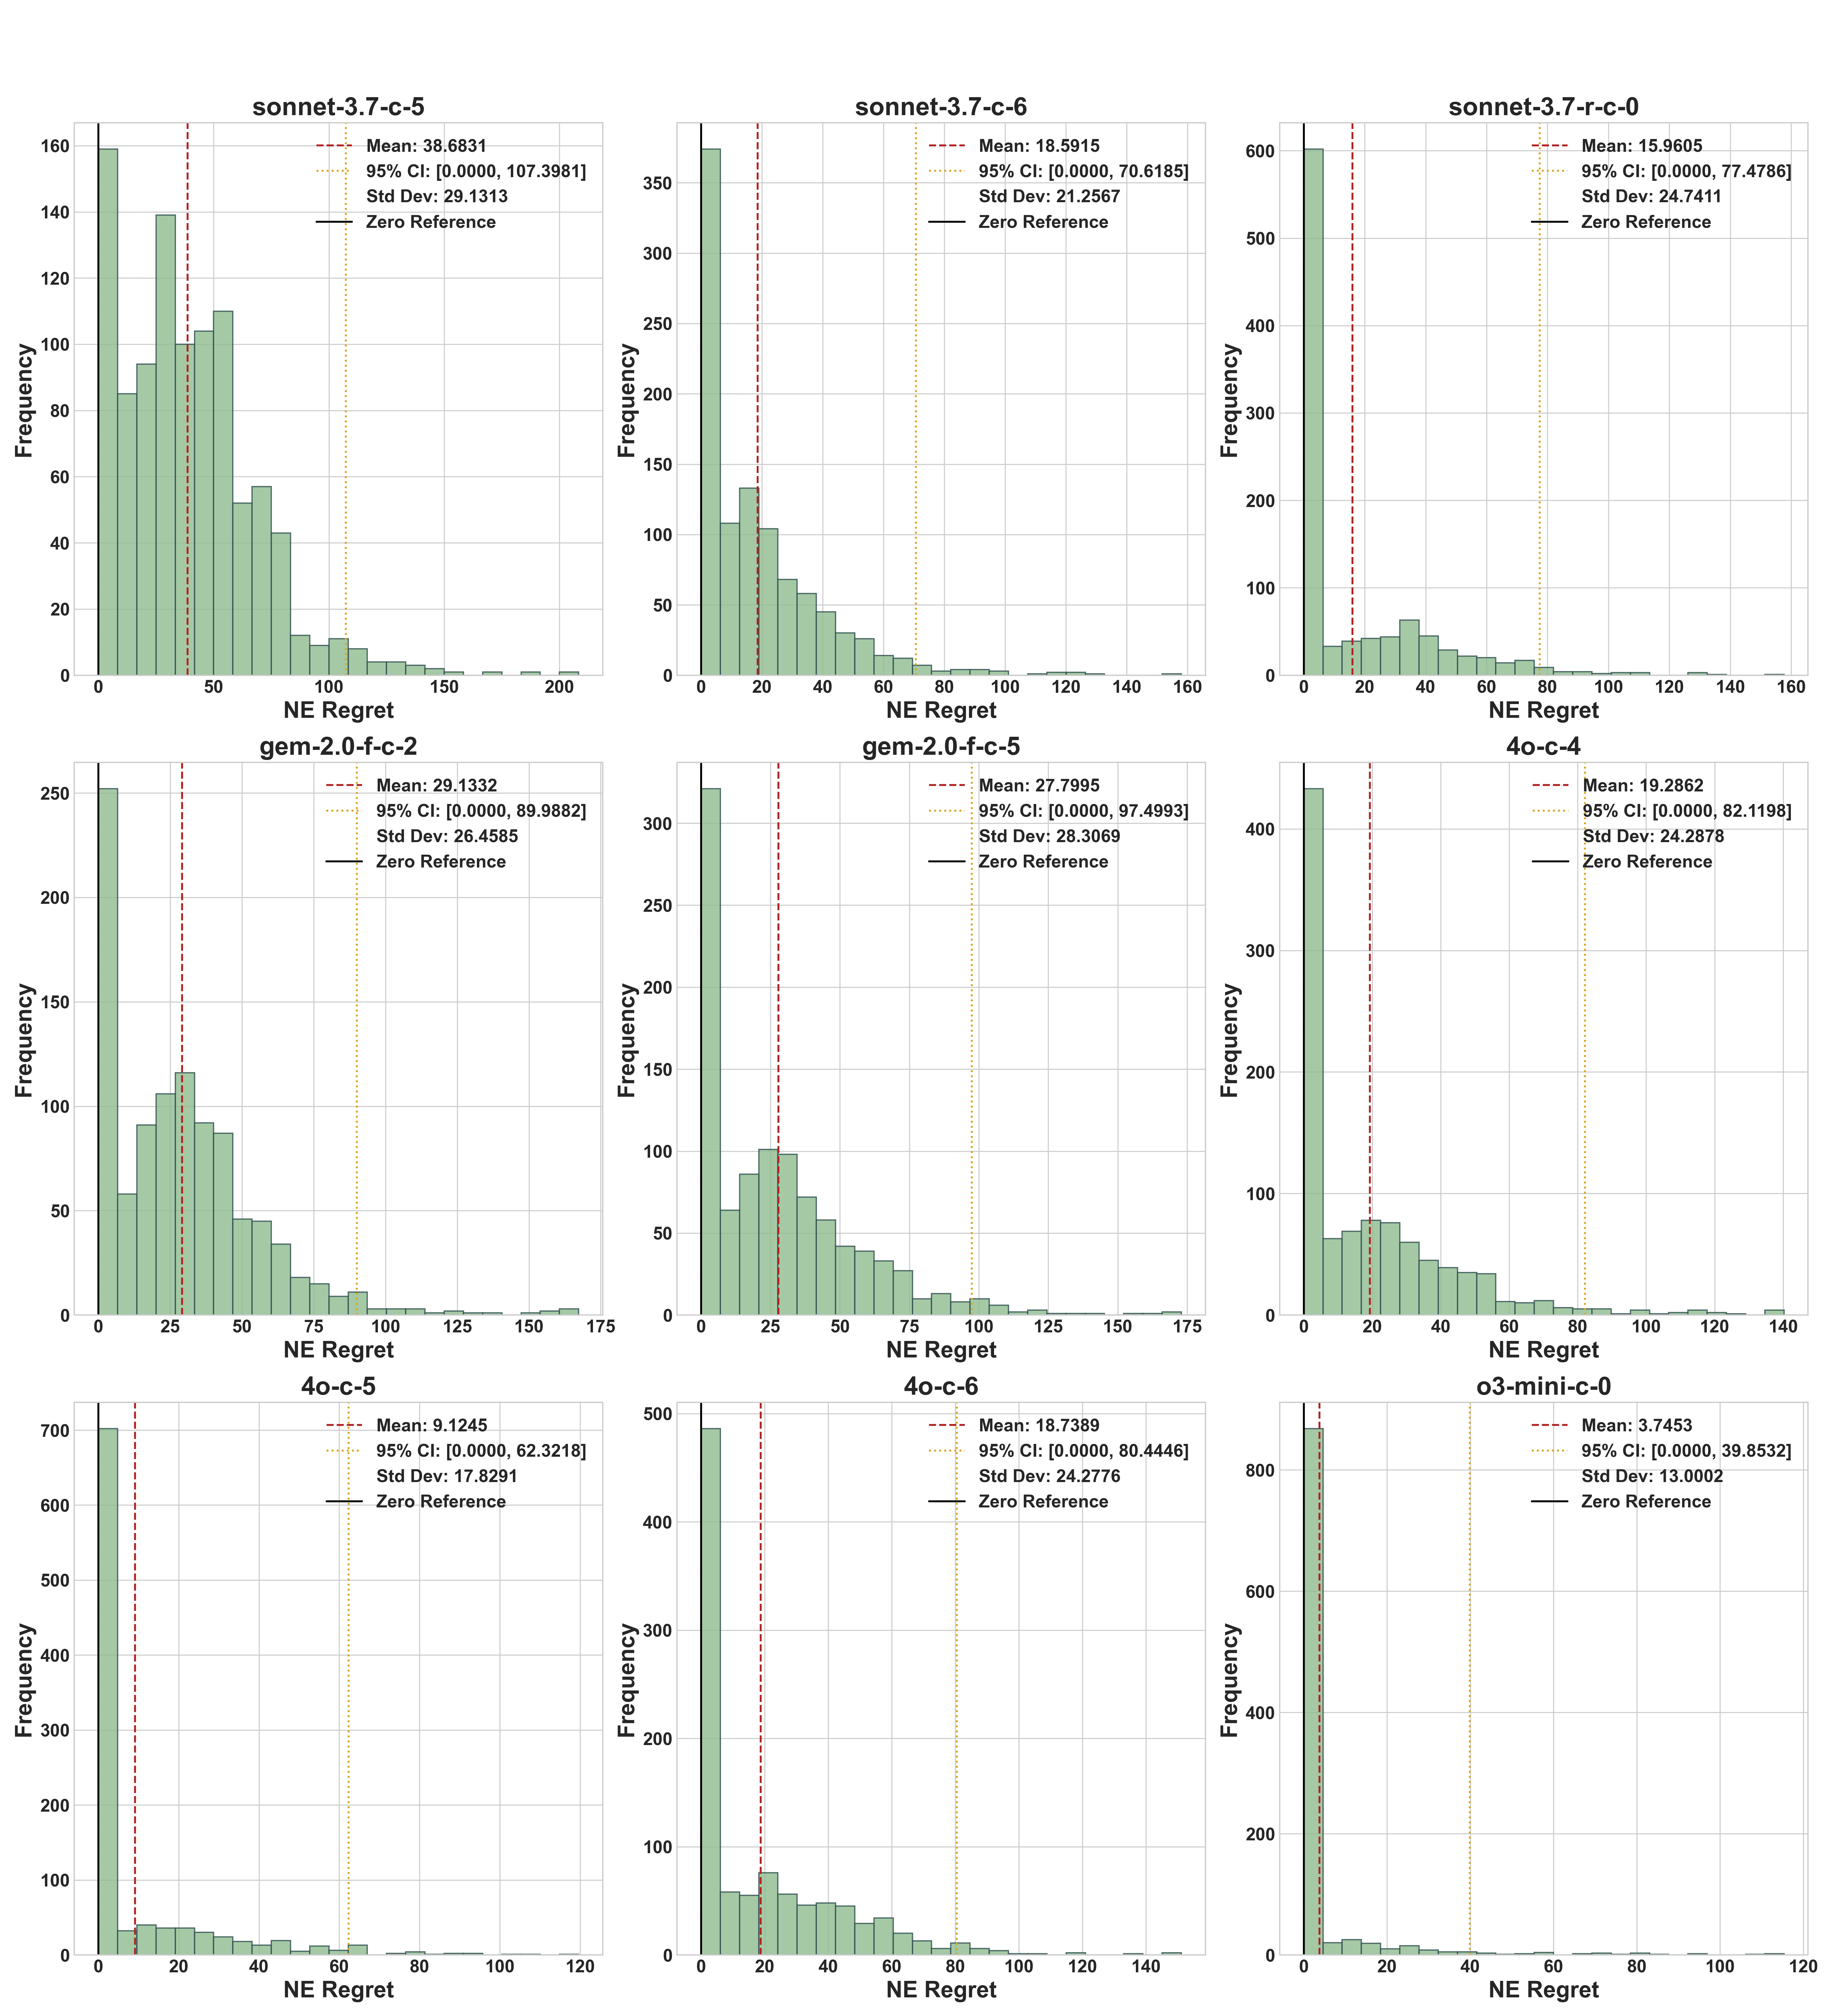
\includegraphics[width=0.46\textwidth]{icml_2025_workshop/bootstrap_distributions/llm_only/game_matrix_2/me_ne_regret.png} &
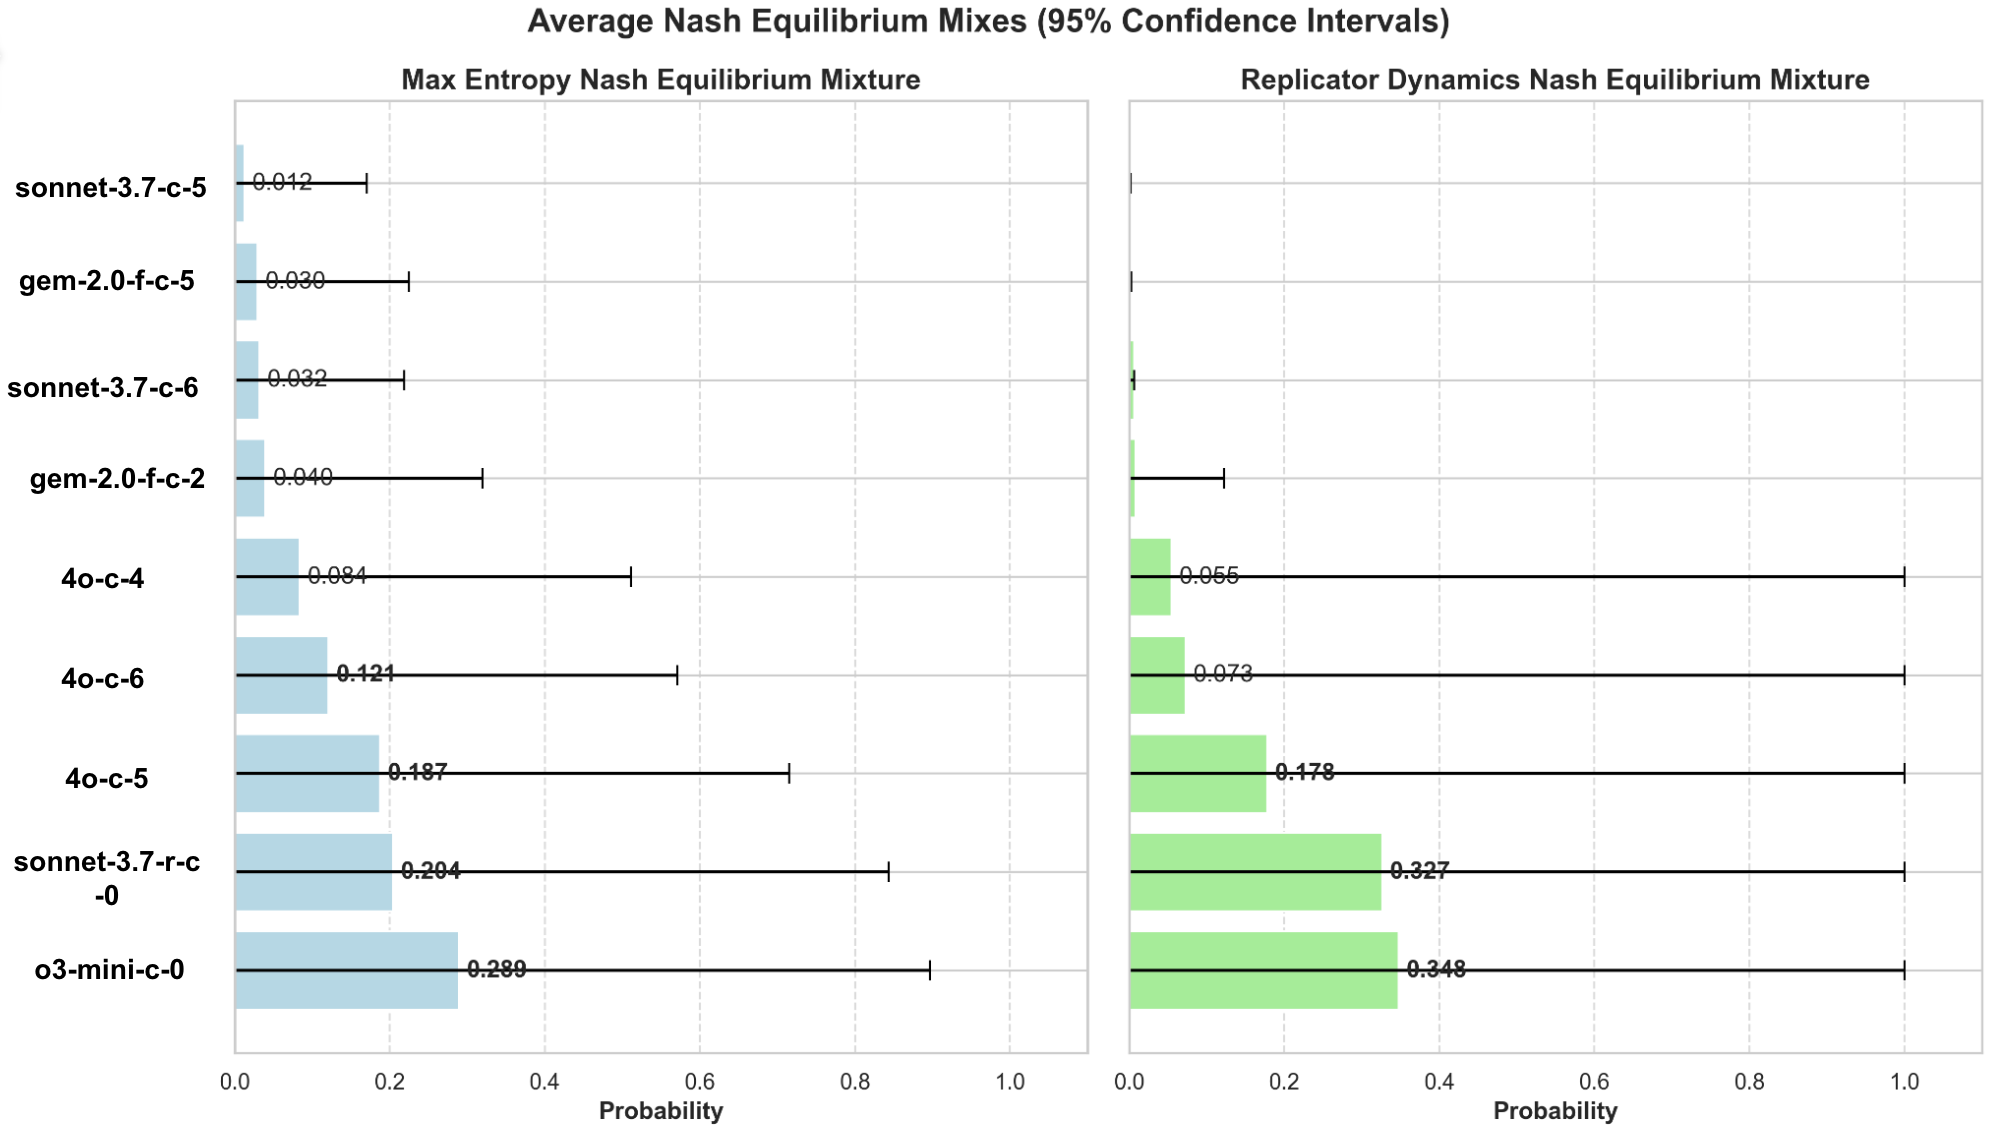
\includegraphics[width=0.46\textwidth]{icml_2025_workshop/bootstrap_distributions/llm_only/game_matrix_2/nash_mixture.png} \\
{\small ME-NE Regret} & {\small Nash Mixture}
\end{tabular}
\caption{LLM-only bootstrap distributions for BG1 and BG2}
\label{fig:llm_only_bg1_bg2}
\end{figure}

\vspace{0.5cm}

\begin{figure}[H]
\centering
\begin{tabular}{cc}
\multicolumn{2}{c}{\textbf{BG3 (\(\gamma=0.98\), \(R=5\))}} \\
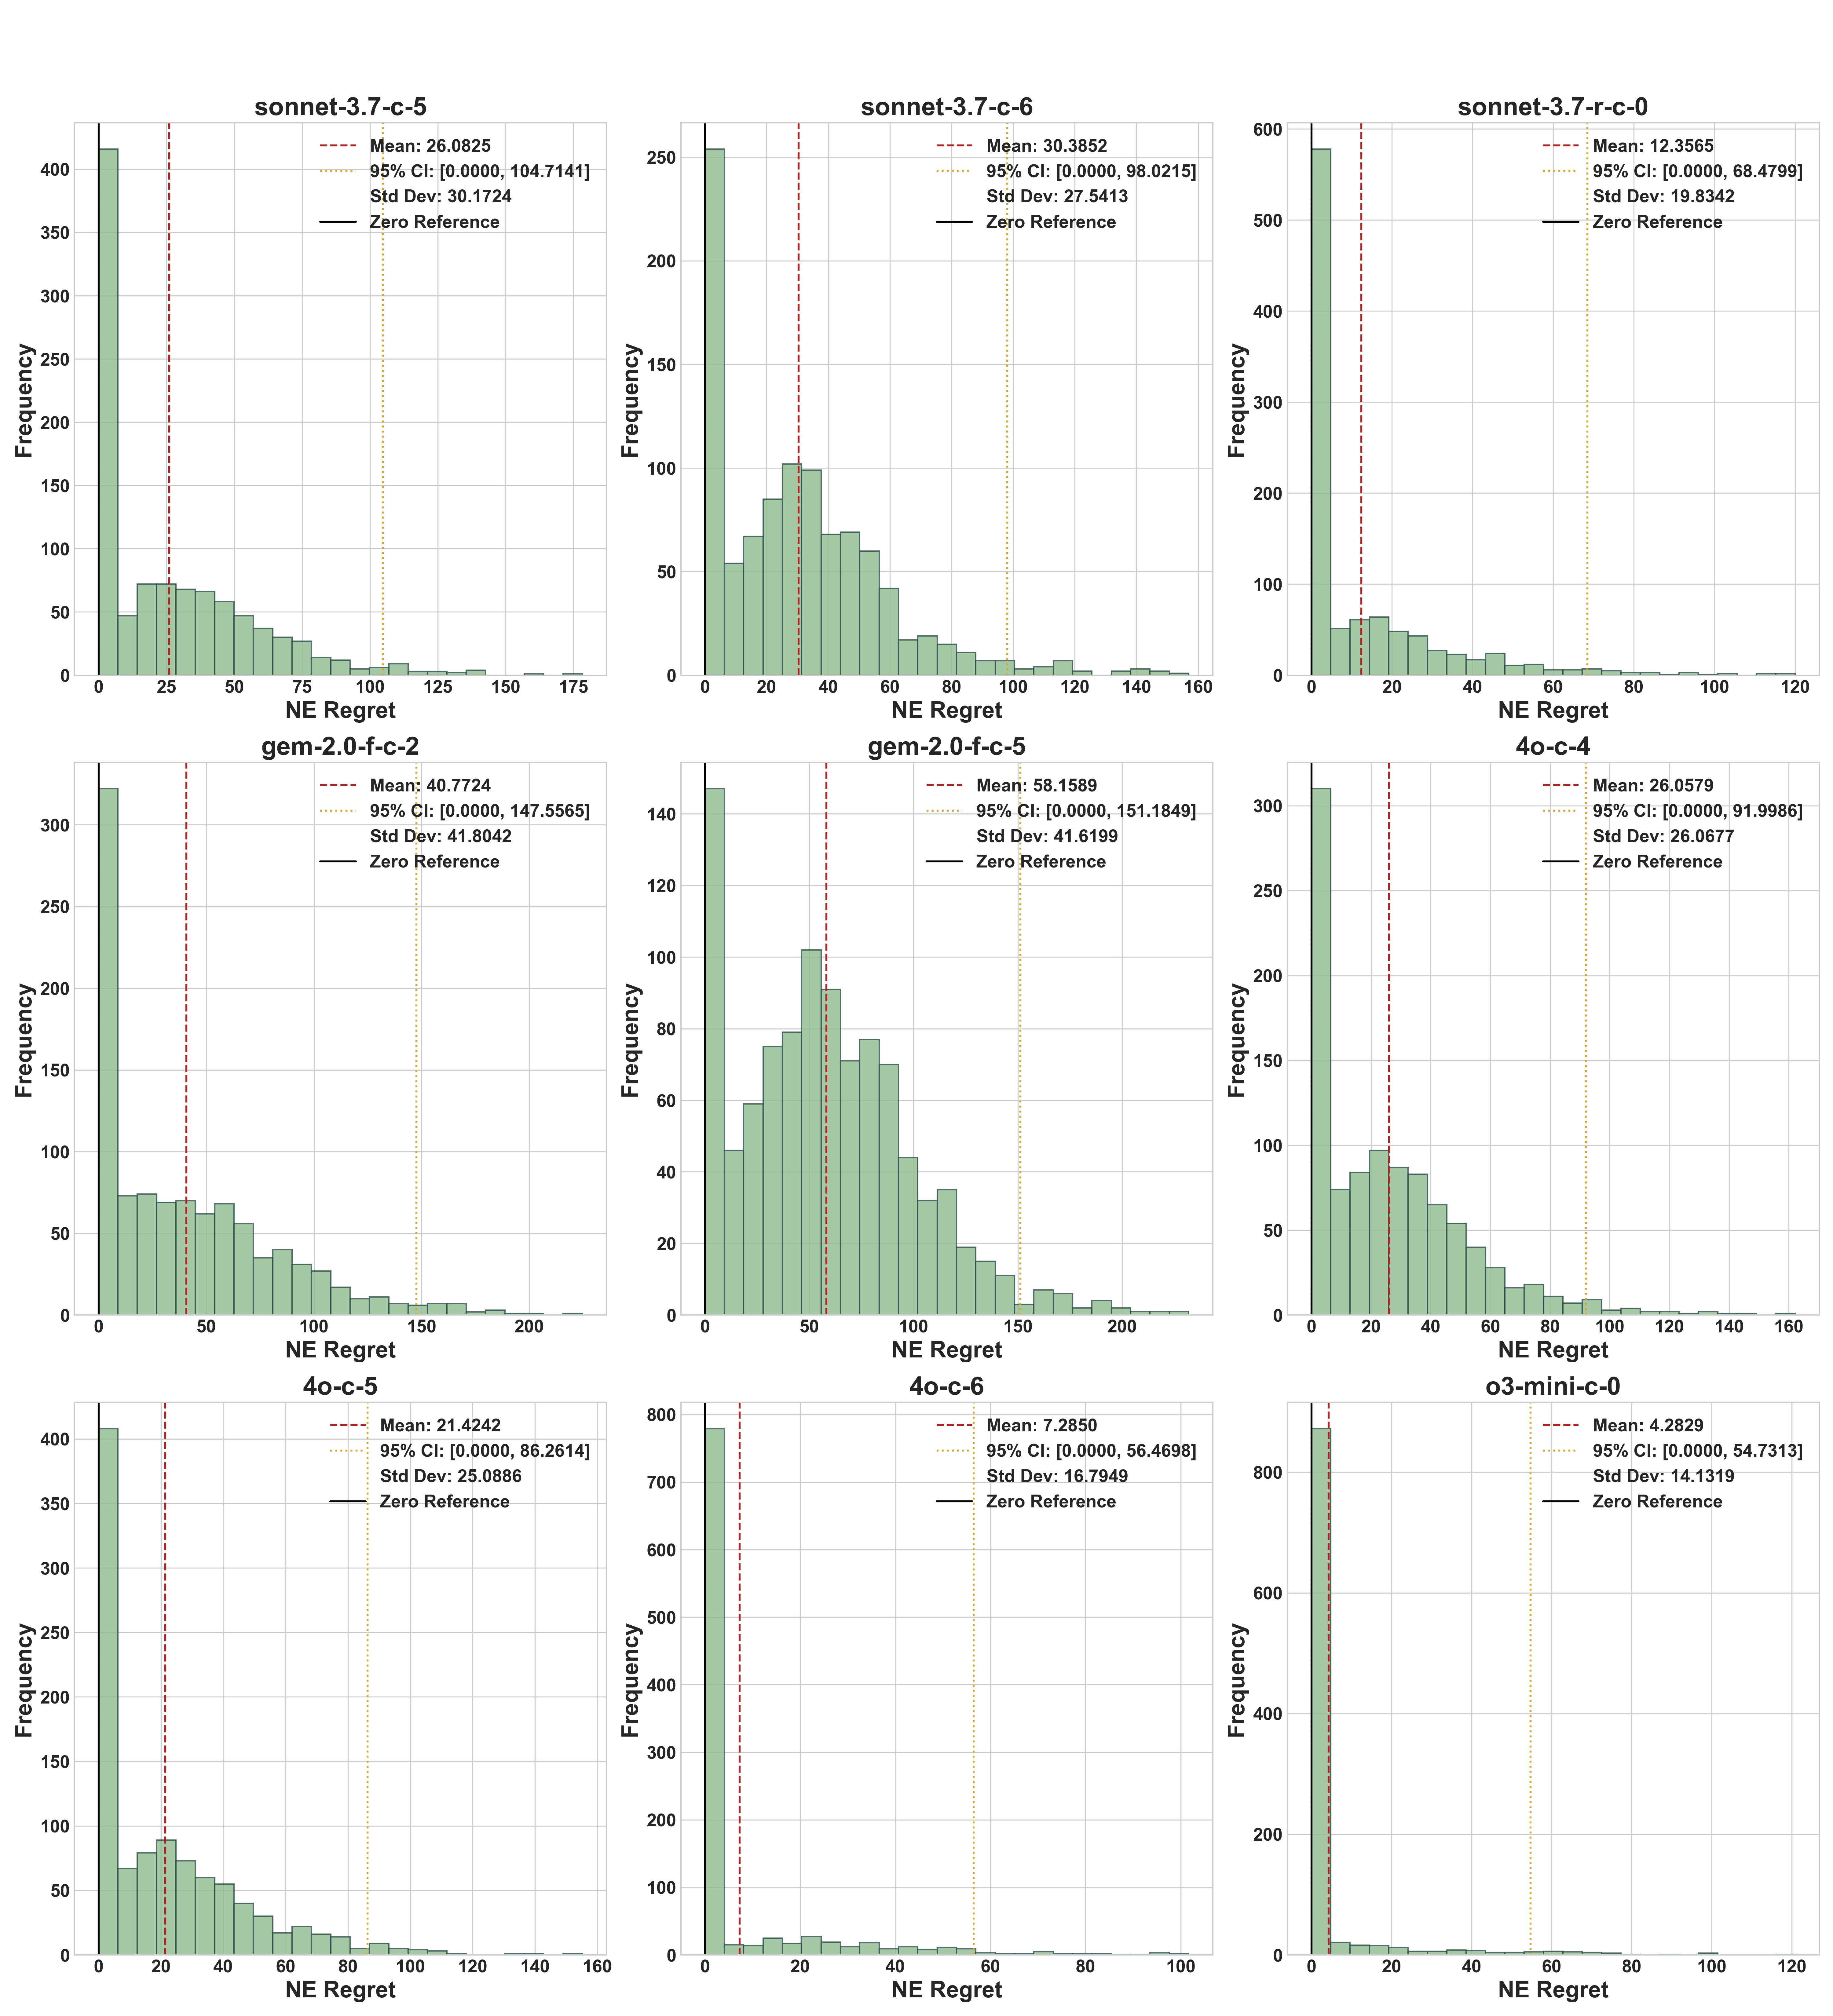
\includegraphics[width=0.46\textwidth]{icml_2025_workshop/bootstrap_distributions/llm_only/game_matrix_3/me_ne_regret.png} &
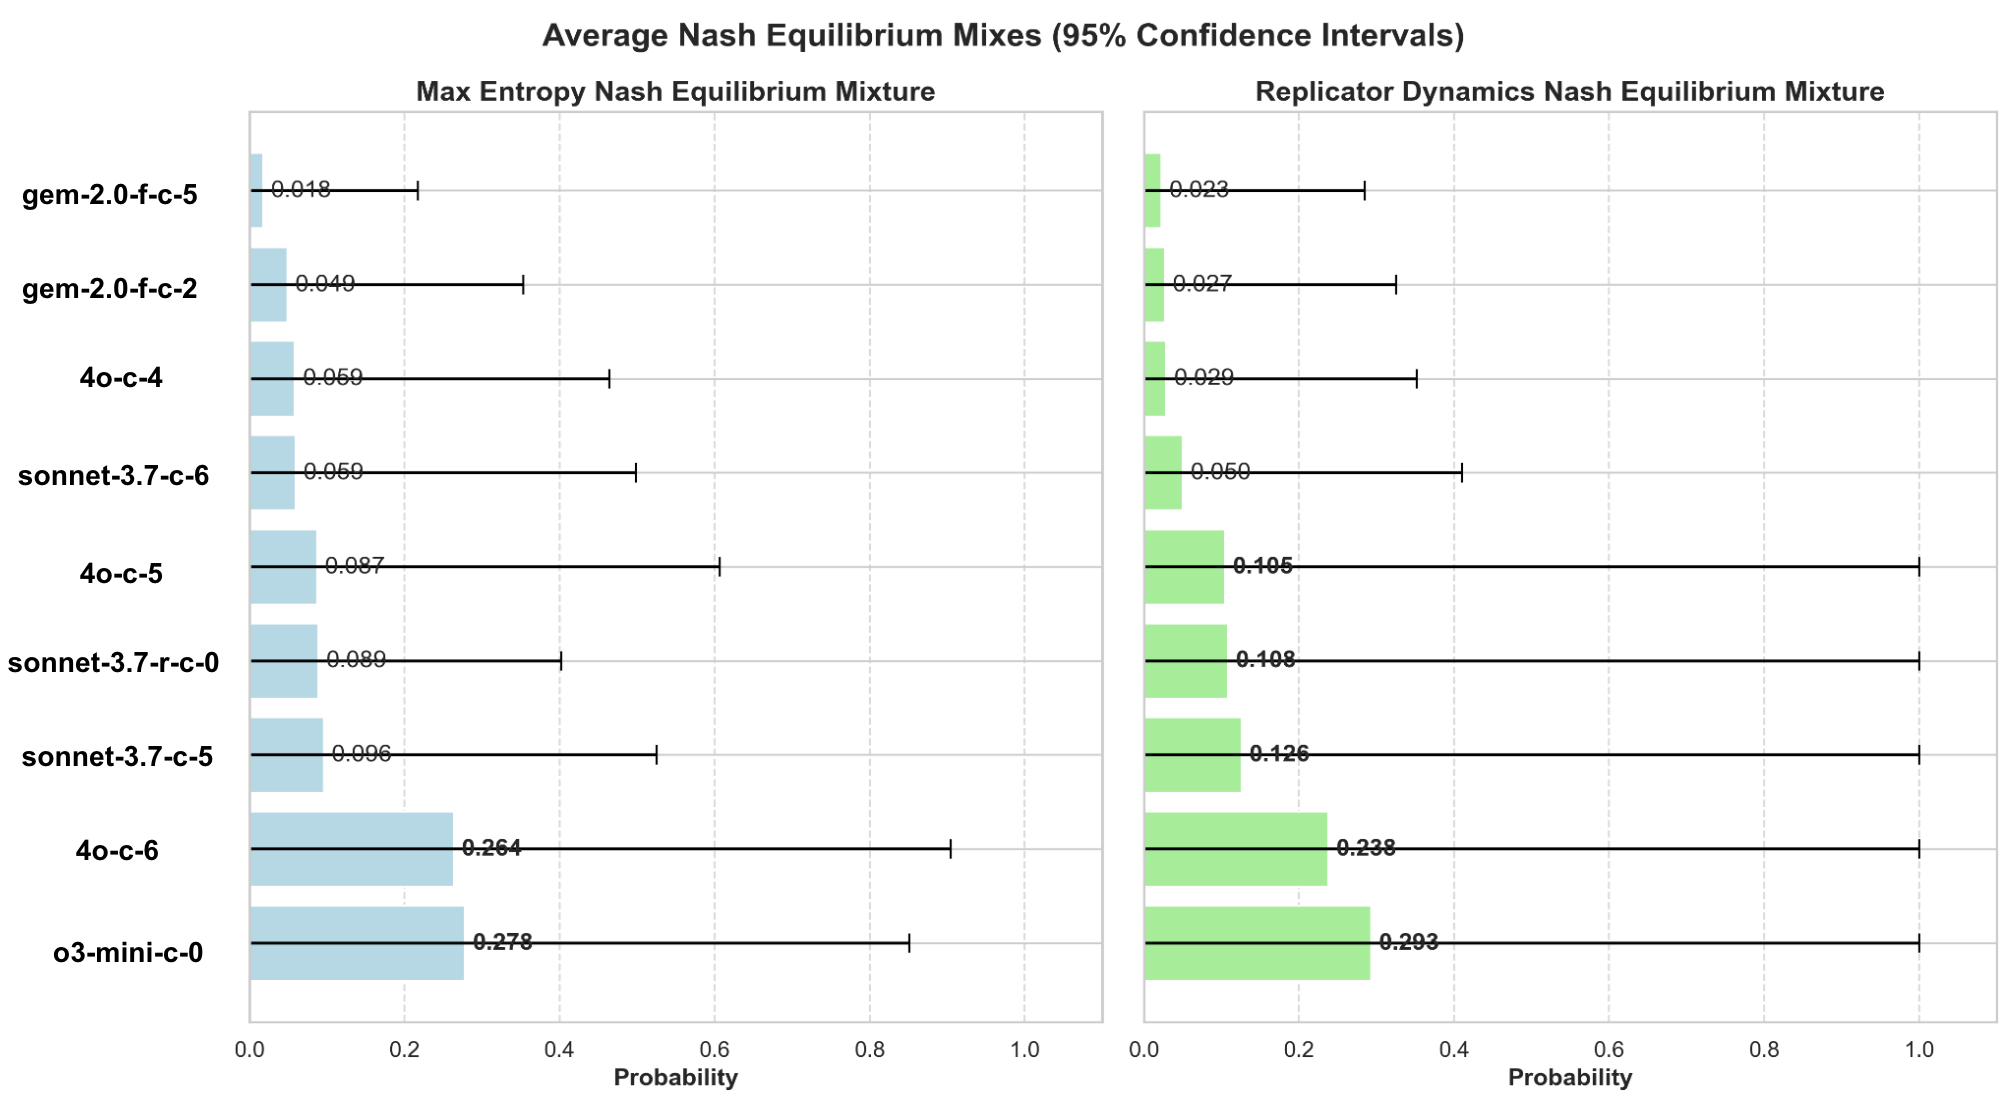
\includegraphics[width=0.46\textwidth]{icml_2025_workshop/bootstrap_distributions/llm_only/game_matrix_3/nash_mixture.png} \\
{\small ME-NE Regret} & {\small Nash Mixture} \\%[0.5cm]

\multicolumn{2}{c}{\textbf{BG0 (meta-game over BG1-BG3)}} \\
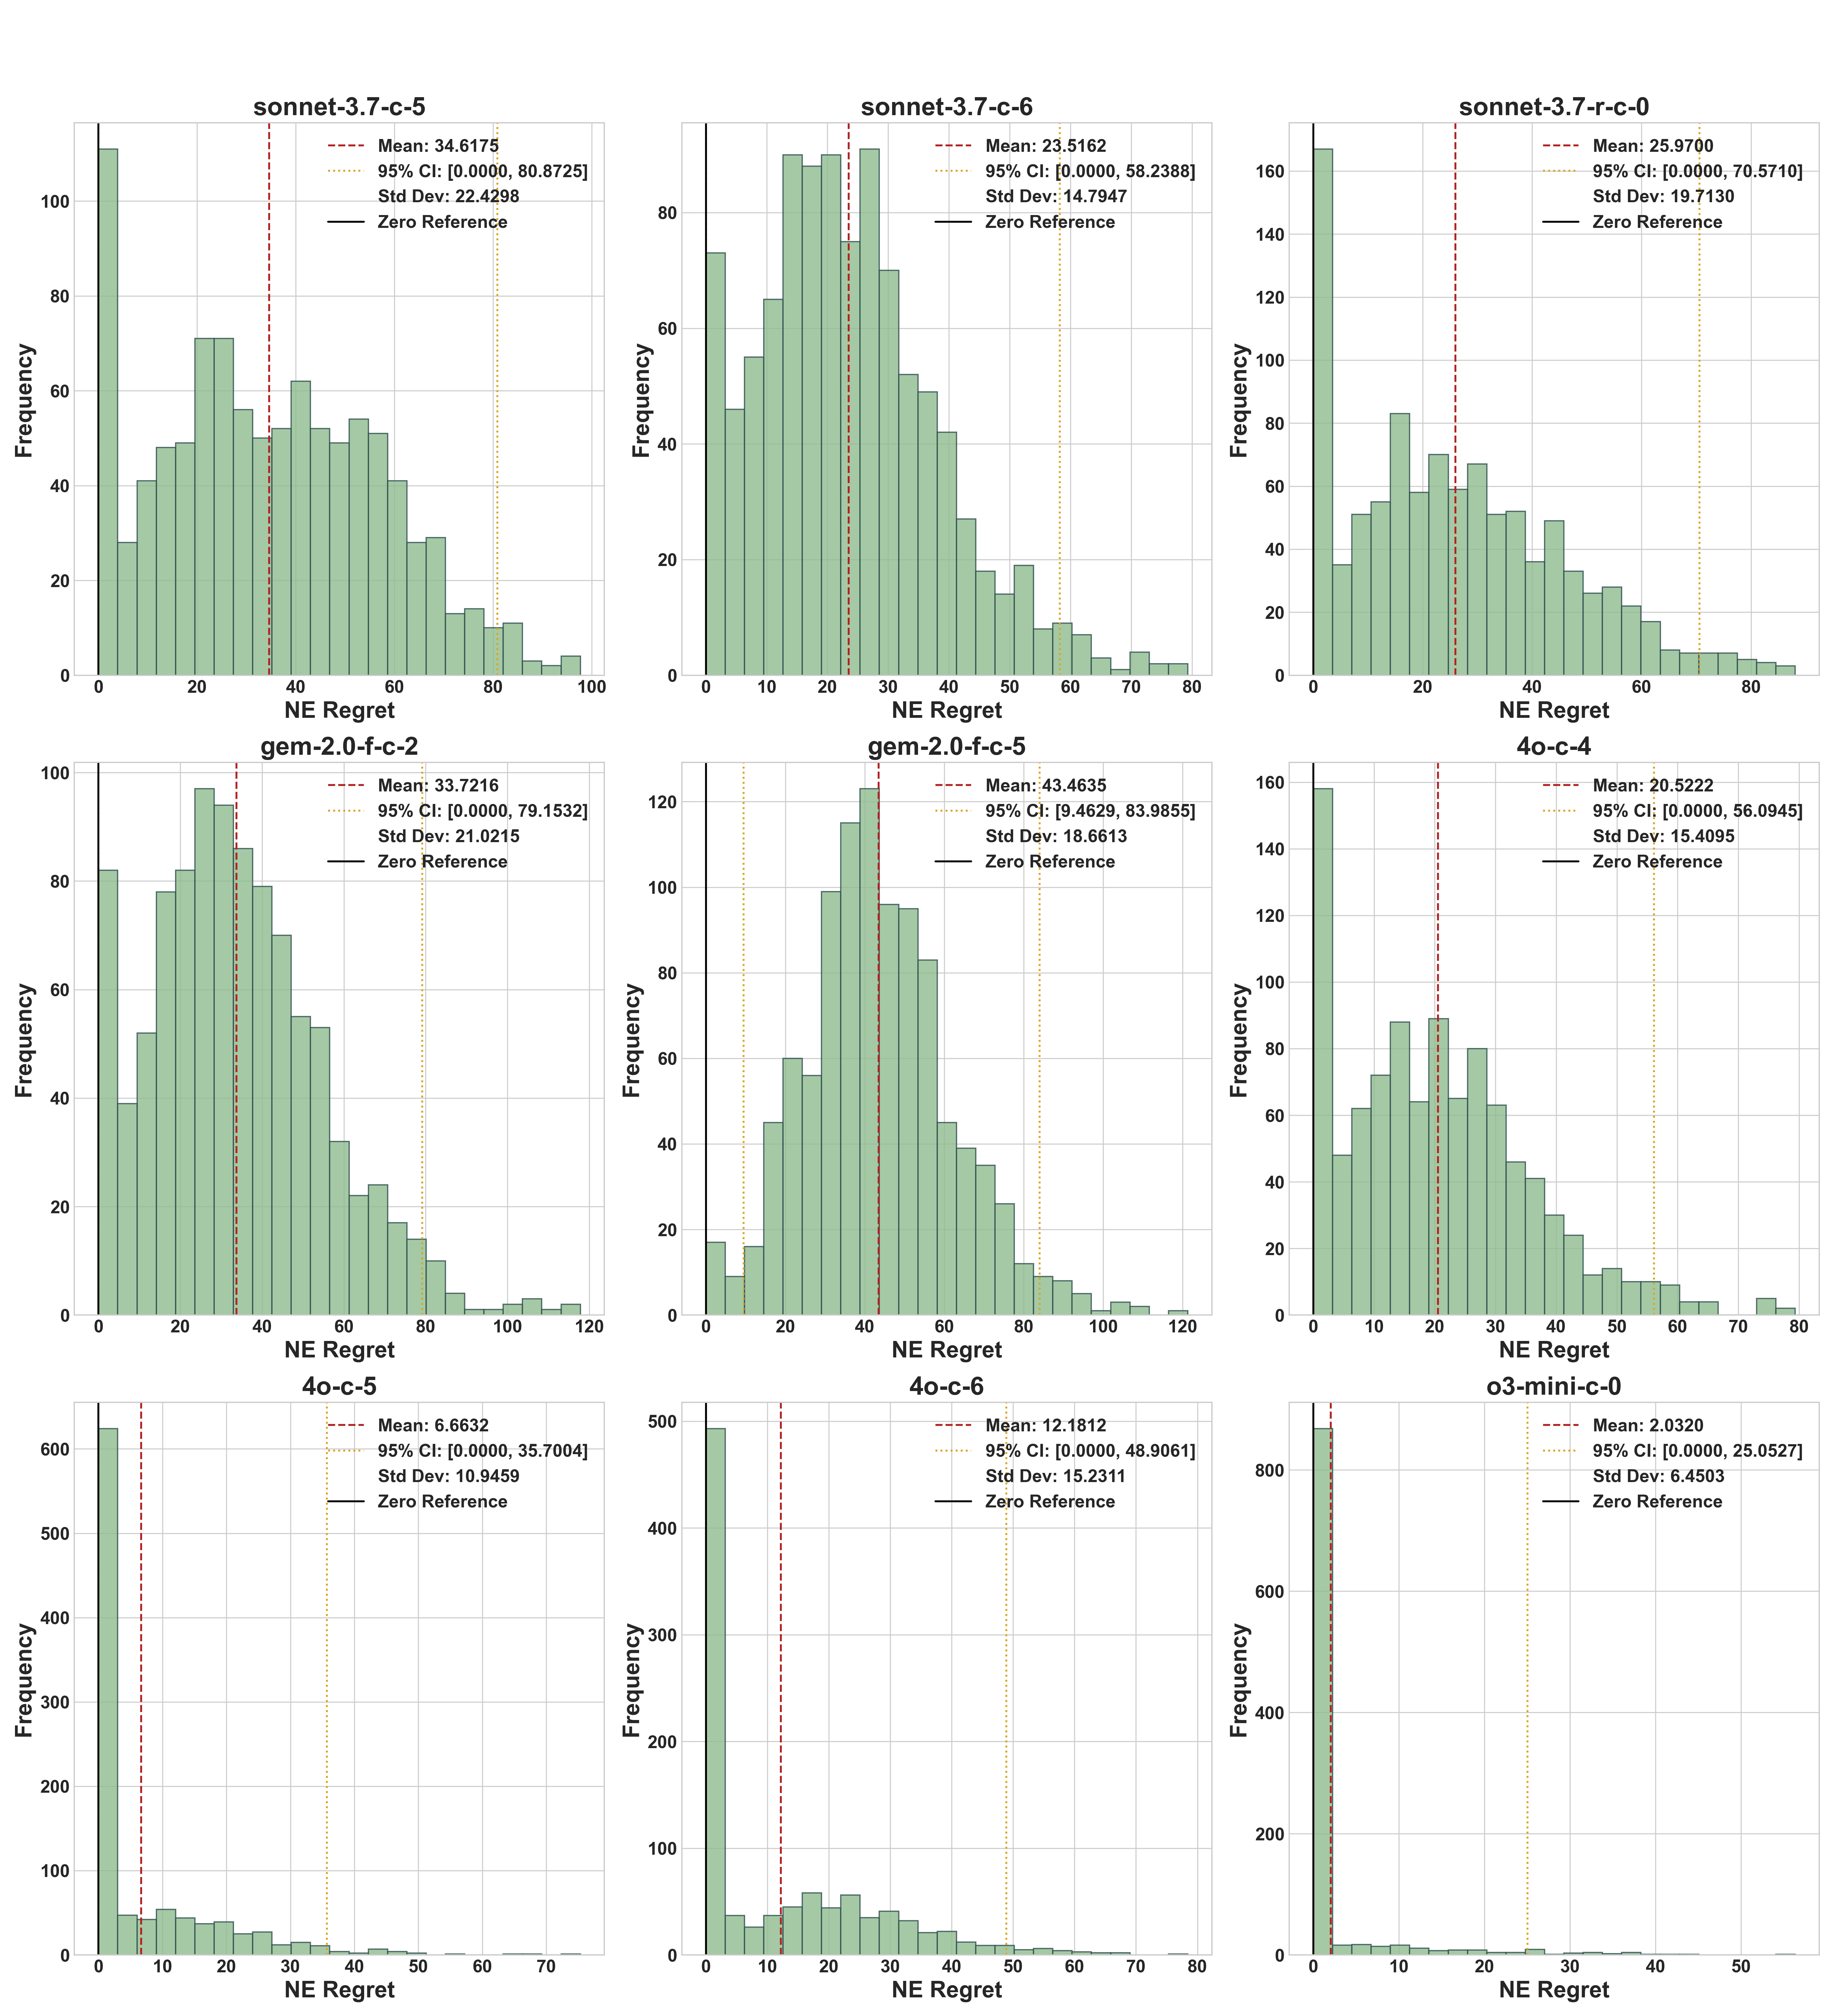
\includegraphics[width=0.46\textwidth]{icml_2025_workshop/bootstrap_distributions/llm_only/game_matrix_4/me_ne_regret.png} &
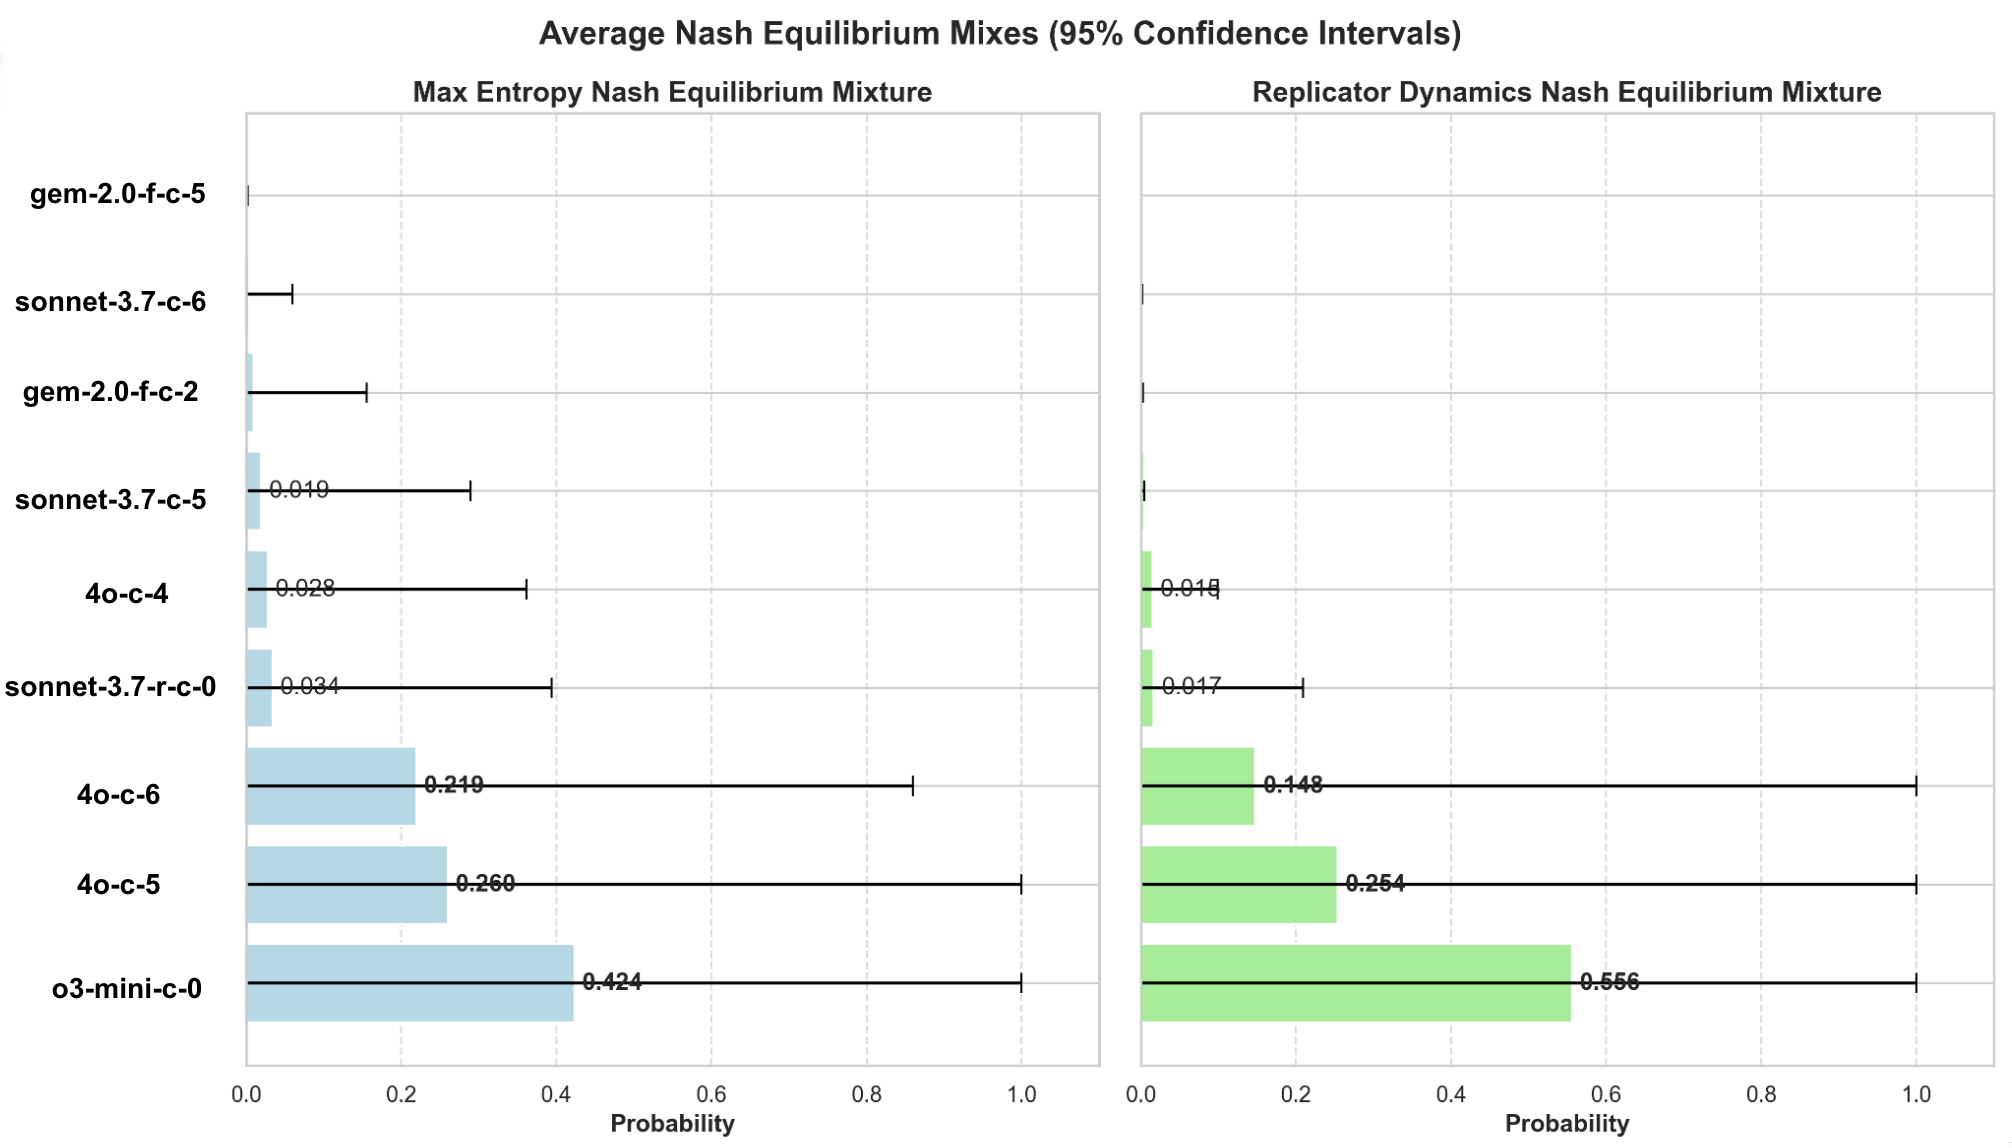
\includegraphics[width=0.46\textwidth]{icml_2025_workshop/bootstrap_distributions/llm_only/game_matrix_4/nash_mixture.png} \\
{\small ME-NE Regret} & {\small Nash Mixture}
\end{tabular}
\caption{LLM-only bootstrap distributions for BG3 and BG0}
\label{fig:llm_only_bg3_bg0}
\end{figure}

\section{LLM‐Only Game Results}
\label{app:llm_only}

In this section, we report key strategic metrics for bargaining games played exclusively between LLM agents. For each configuration (BG1–BG3, and the meta-game BG0), we present bootstrap distributions of two core equilibrium metrics computed over 1,000 resamples. Maximum-entropy Nash equilibrium (MENE) regret measures the deviation from equilibrium play. Average Nash equilibrium mixture weights show the distribution of strategies in equilibrium.

\newpage


\begin{figure}[H]
\centering
\begin{tabular}{cc}
\multicolumn{2}{c}{\textbf{BG1 (\(\gamma=0.9\), \(R=3\))}} \\
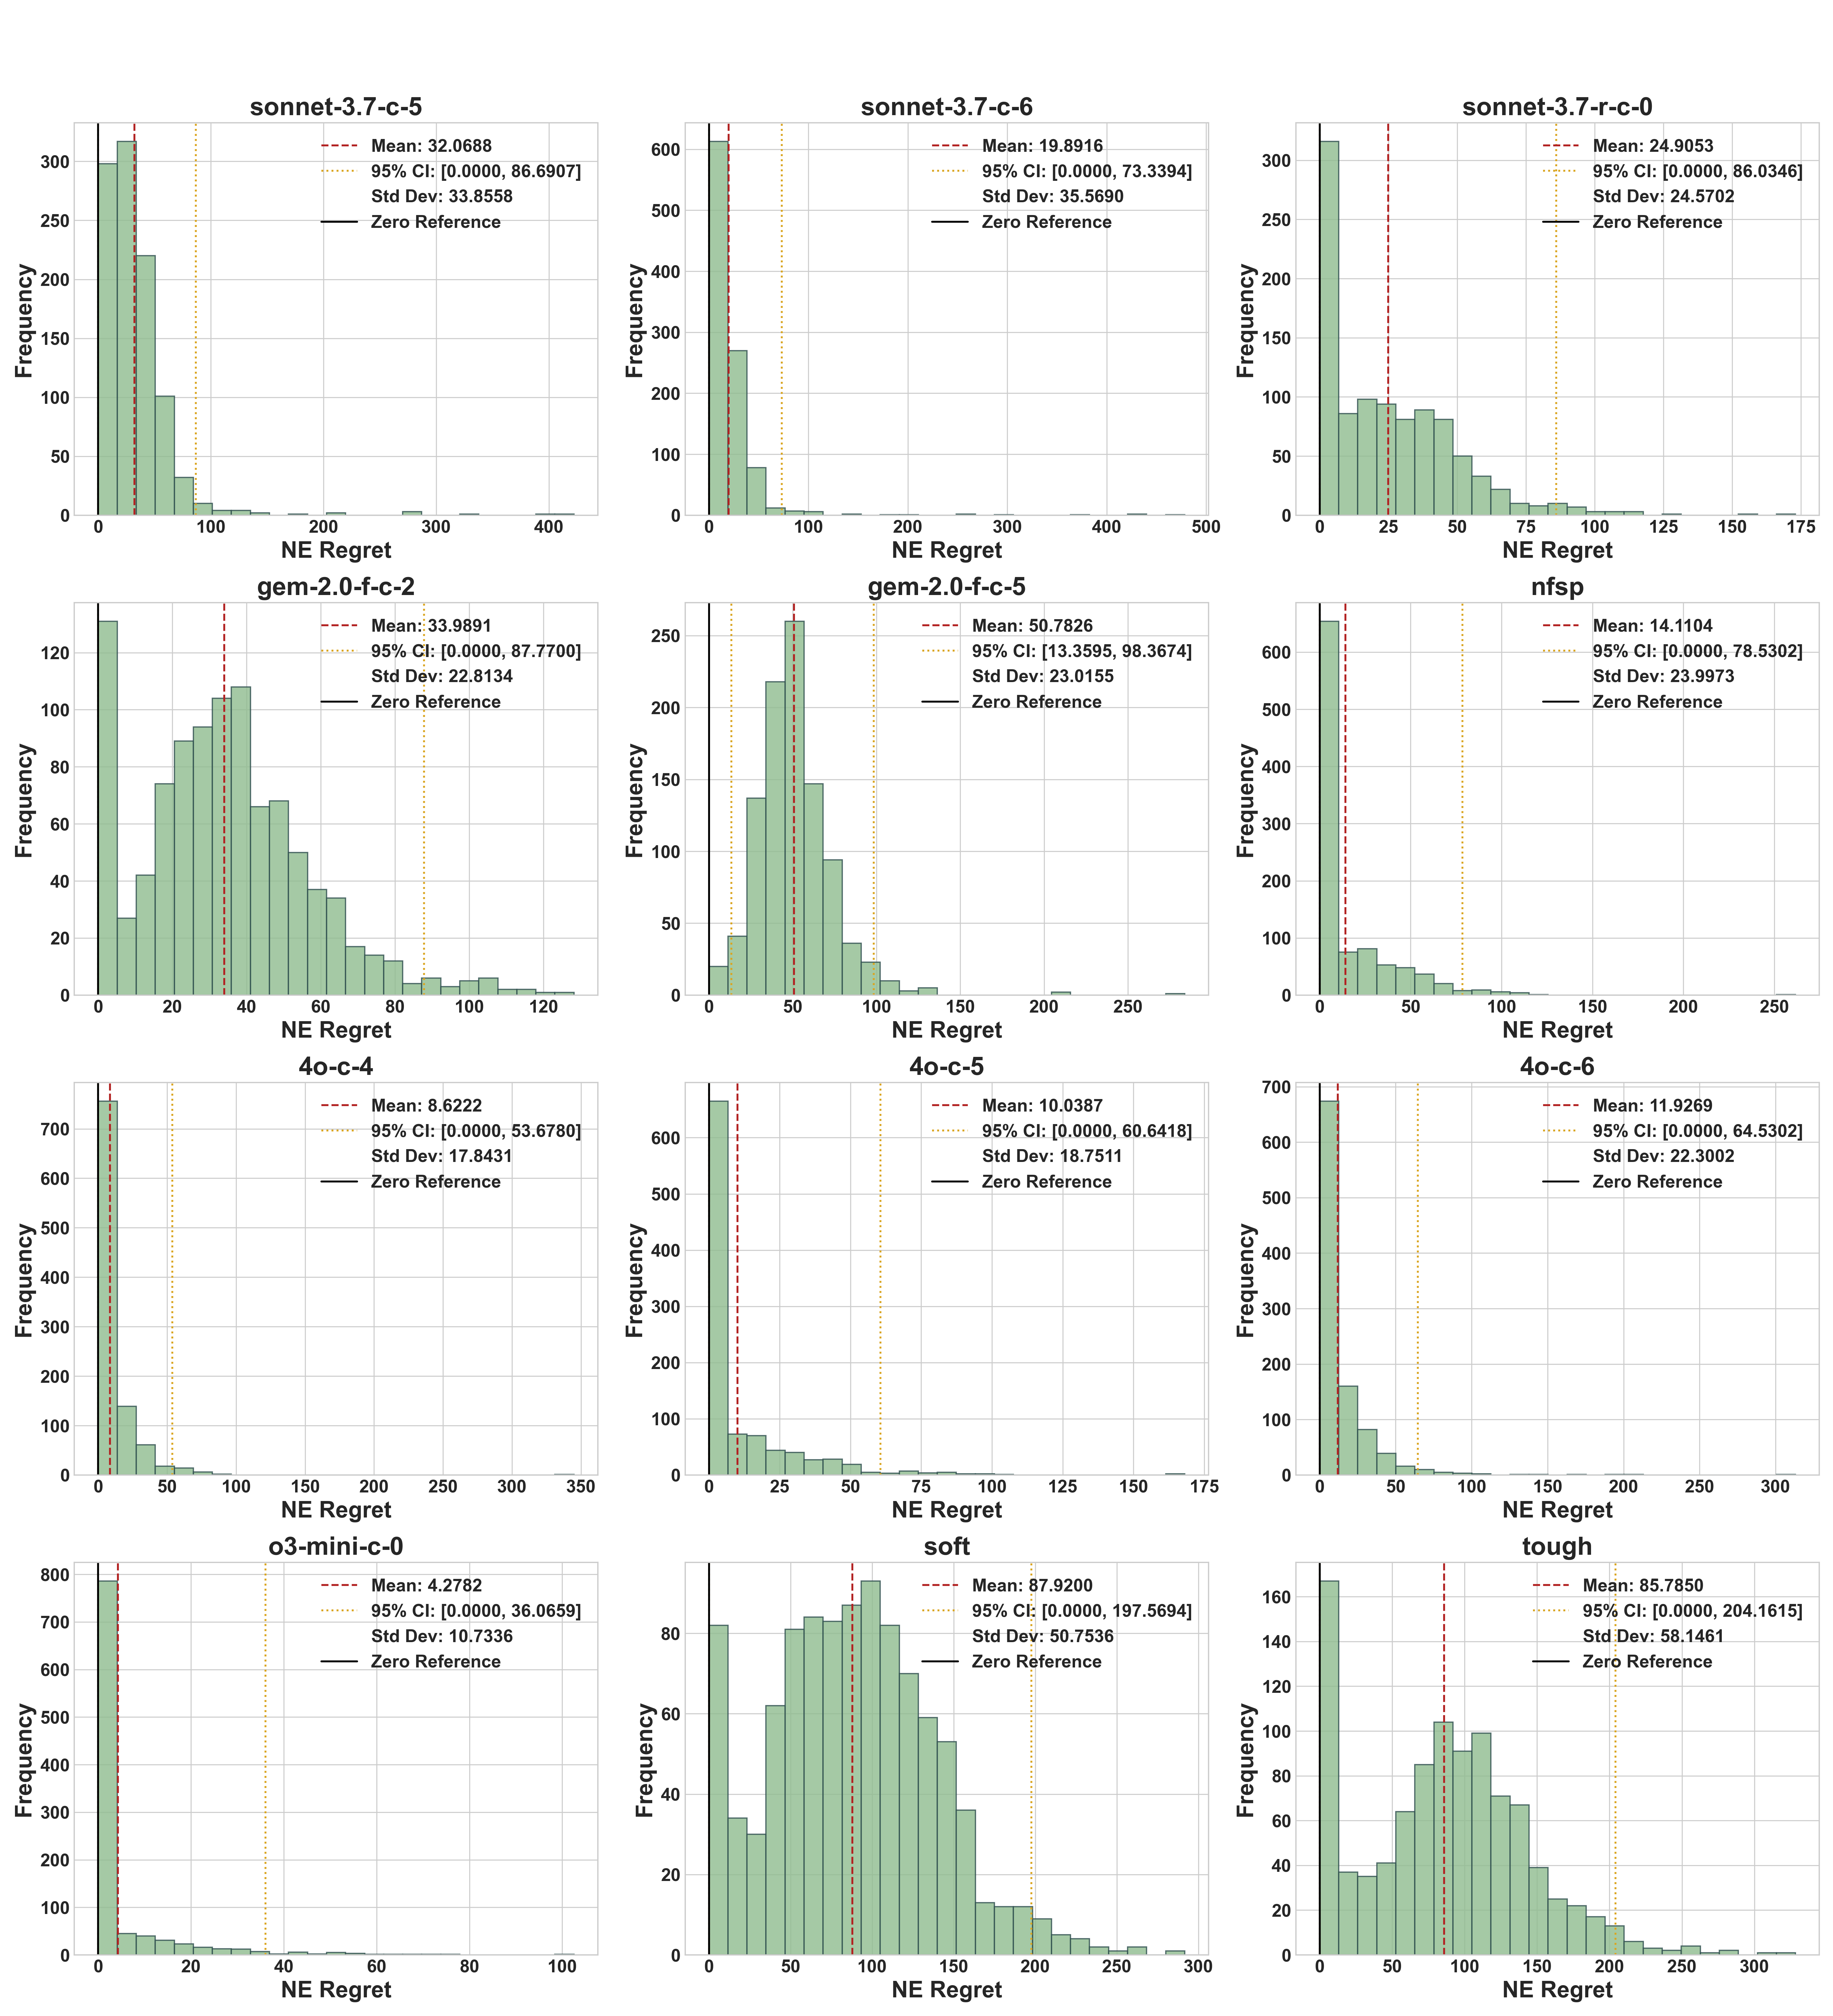
\includegraphics[width=0.46\textwidth]{icml_2025_workshop/bootstrap_distributions/LLM+NonLLM/game_matrix_1/me_ne_regret.png} &
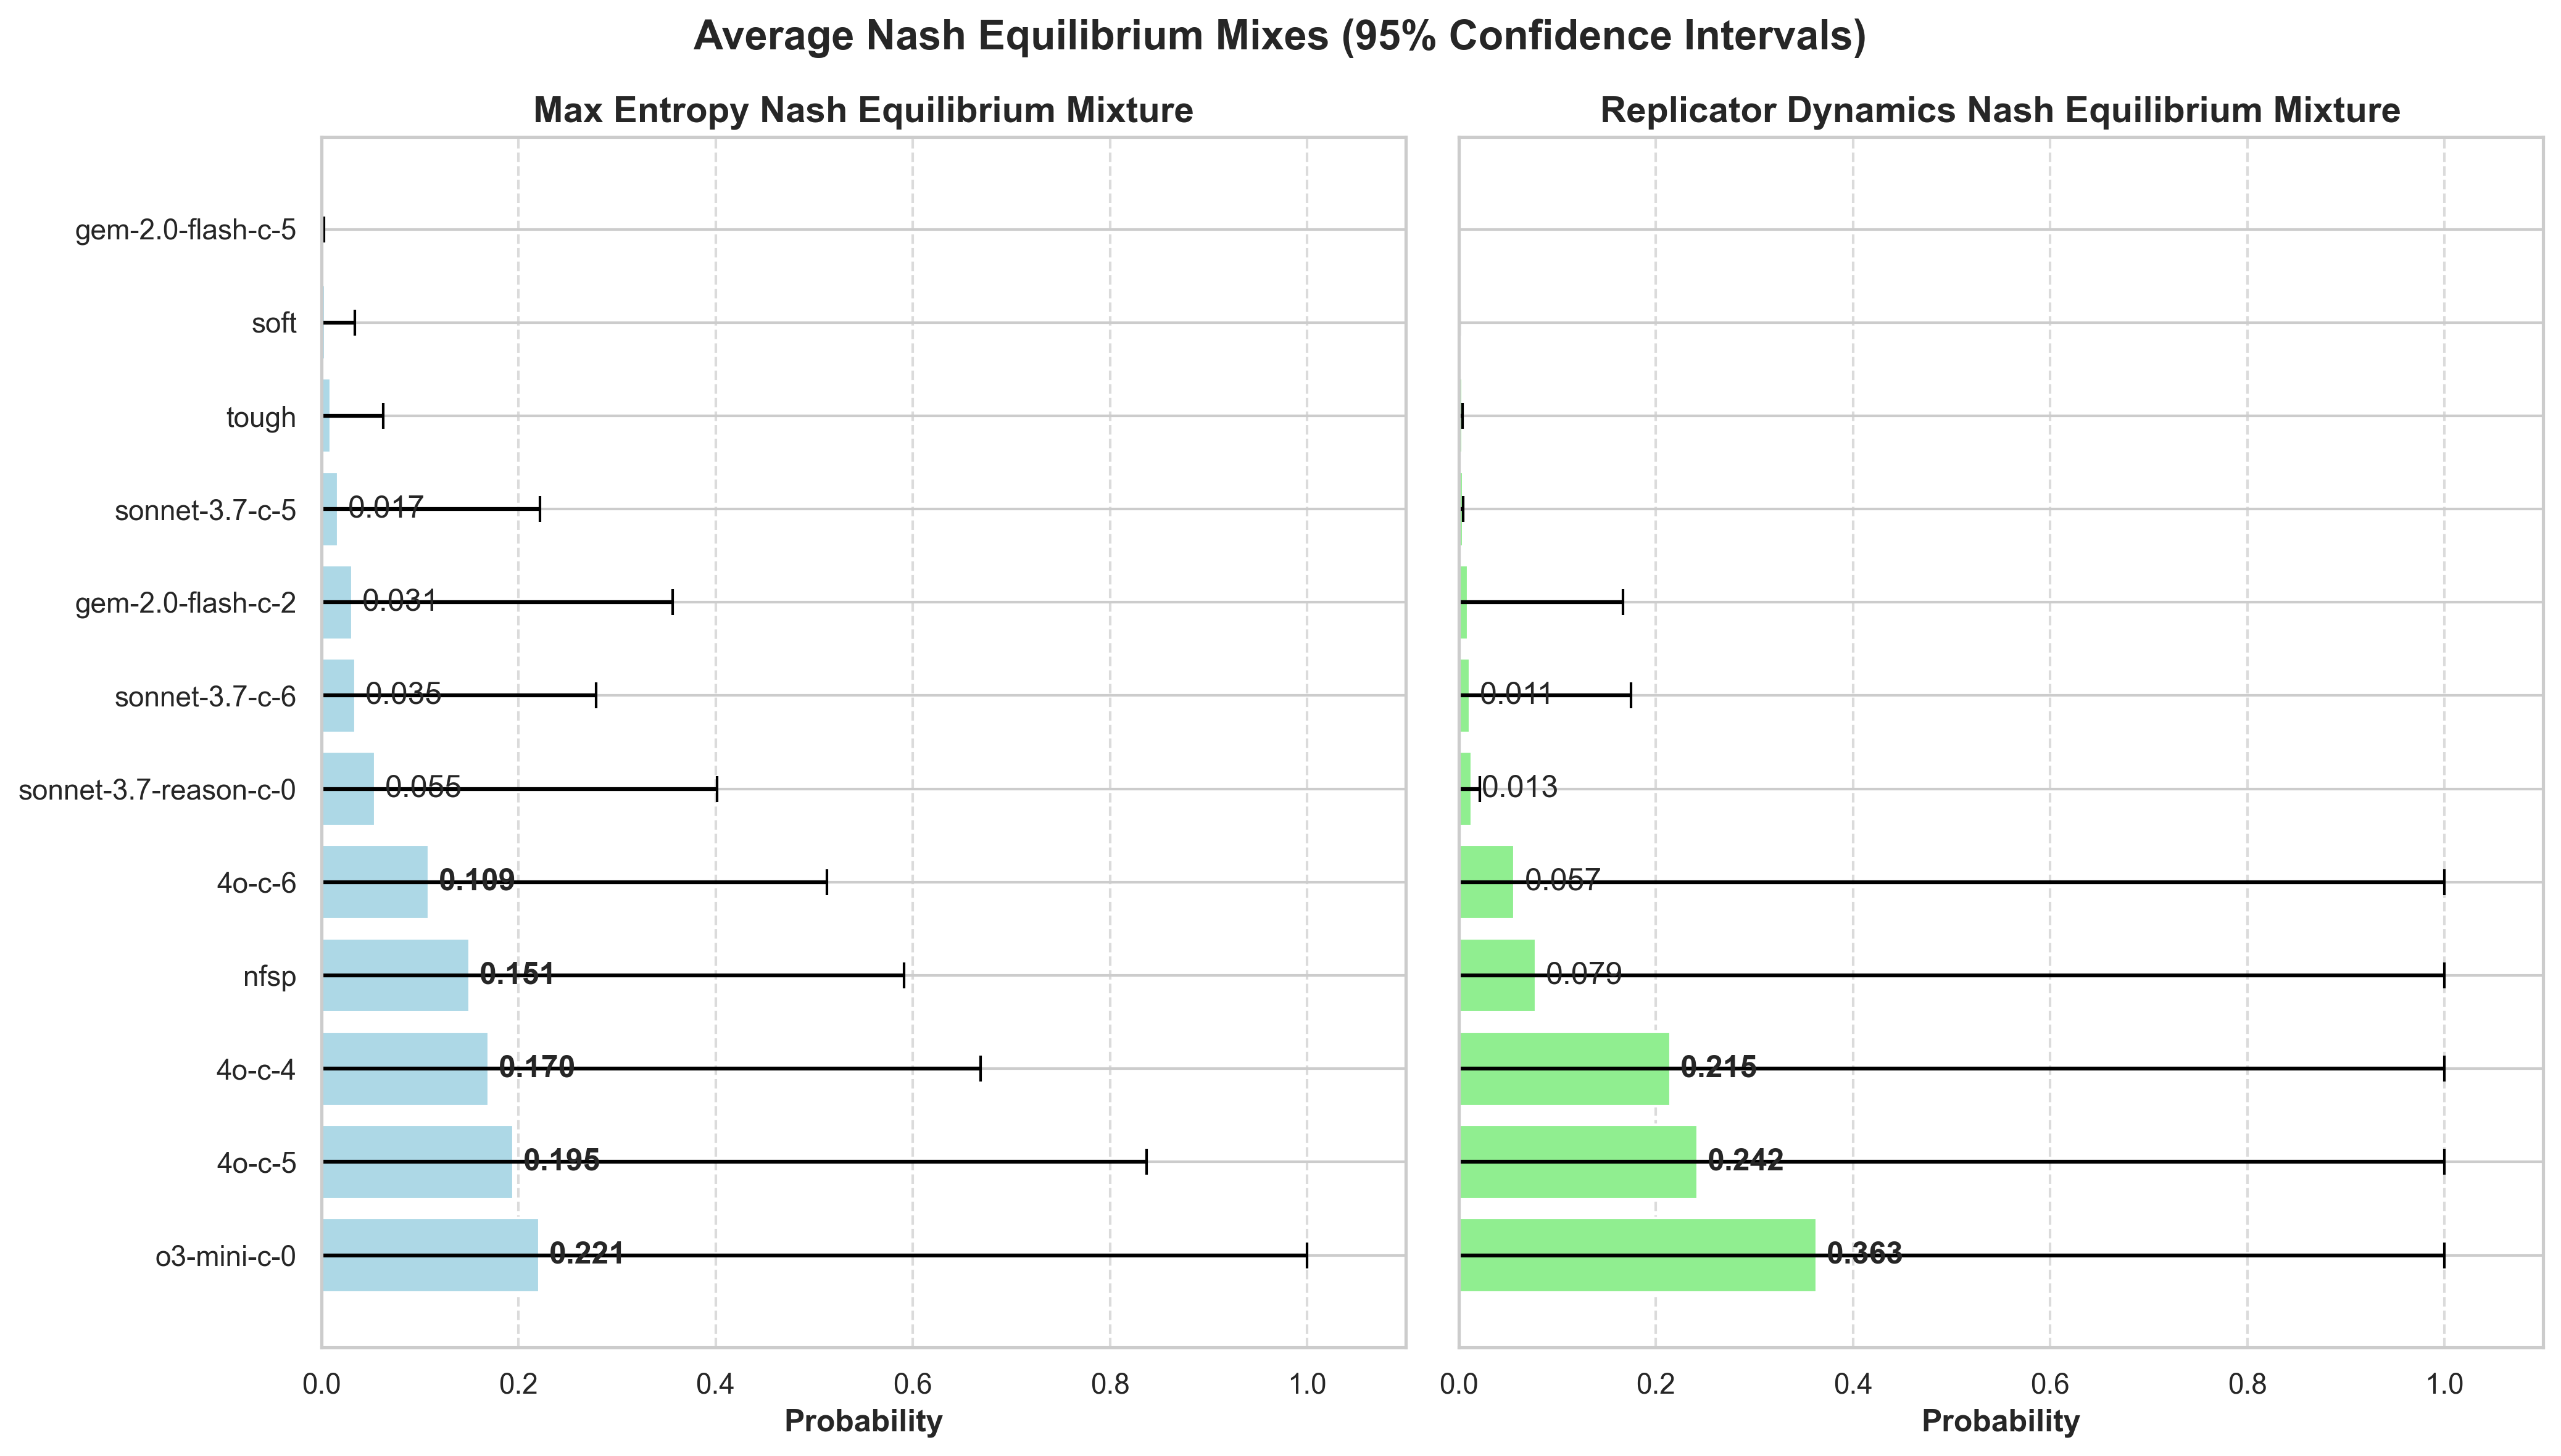
\includegraphics[width=0.46\textwidth]{icml_2025_workshop/bootstrap_distributions/LLM+NonLLM/game_matrix_1/nash_mixture.png} \\
{\small ME-NE Regret} & {\small Nash Mixture} \\%[0.5cm]

\multicolumn{2}{c}{\textbf{BG2 (\(\gamma=0.98\), \(R=3\))}} \\
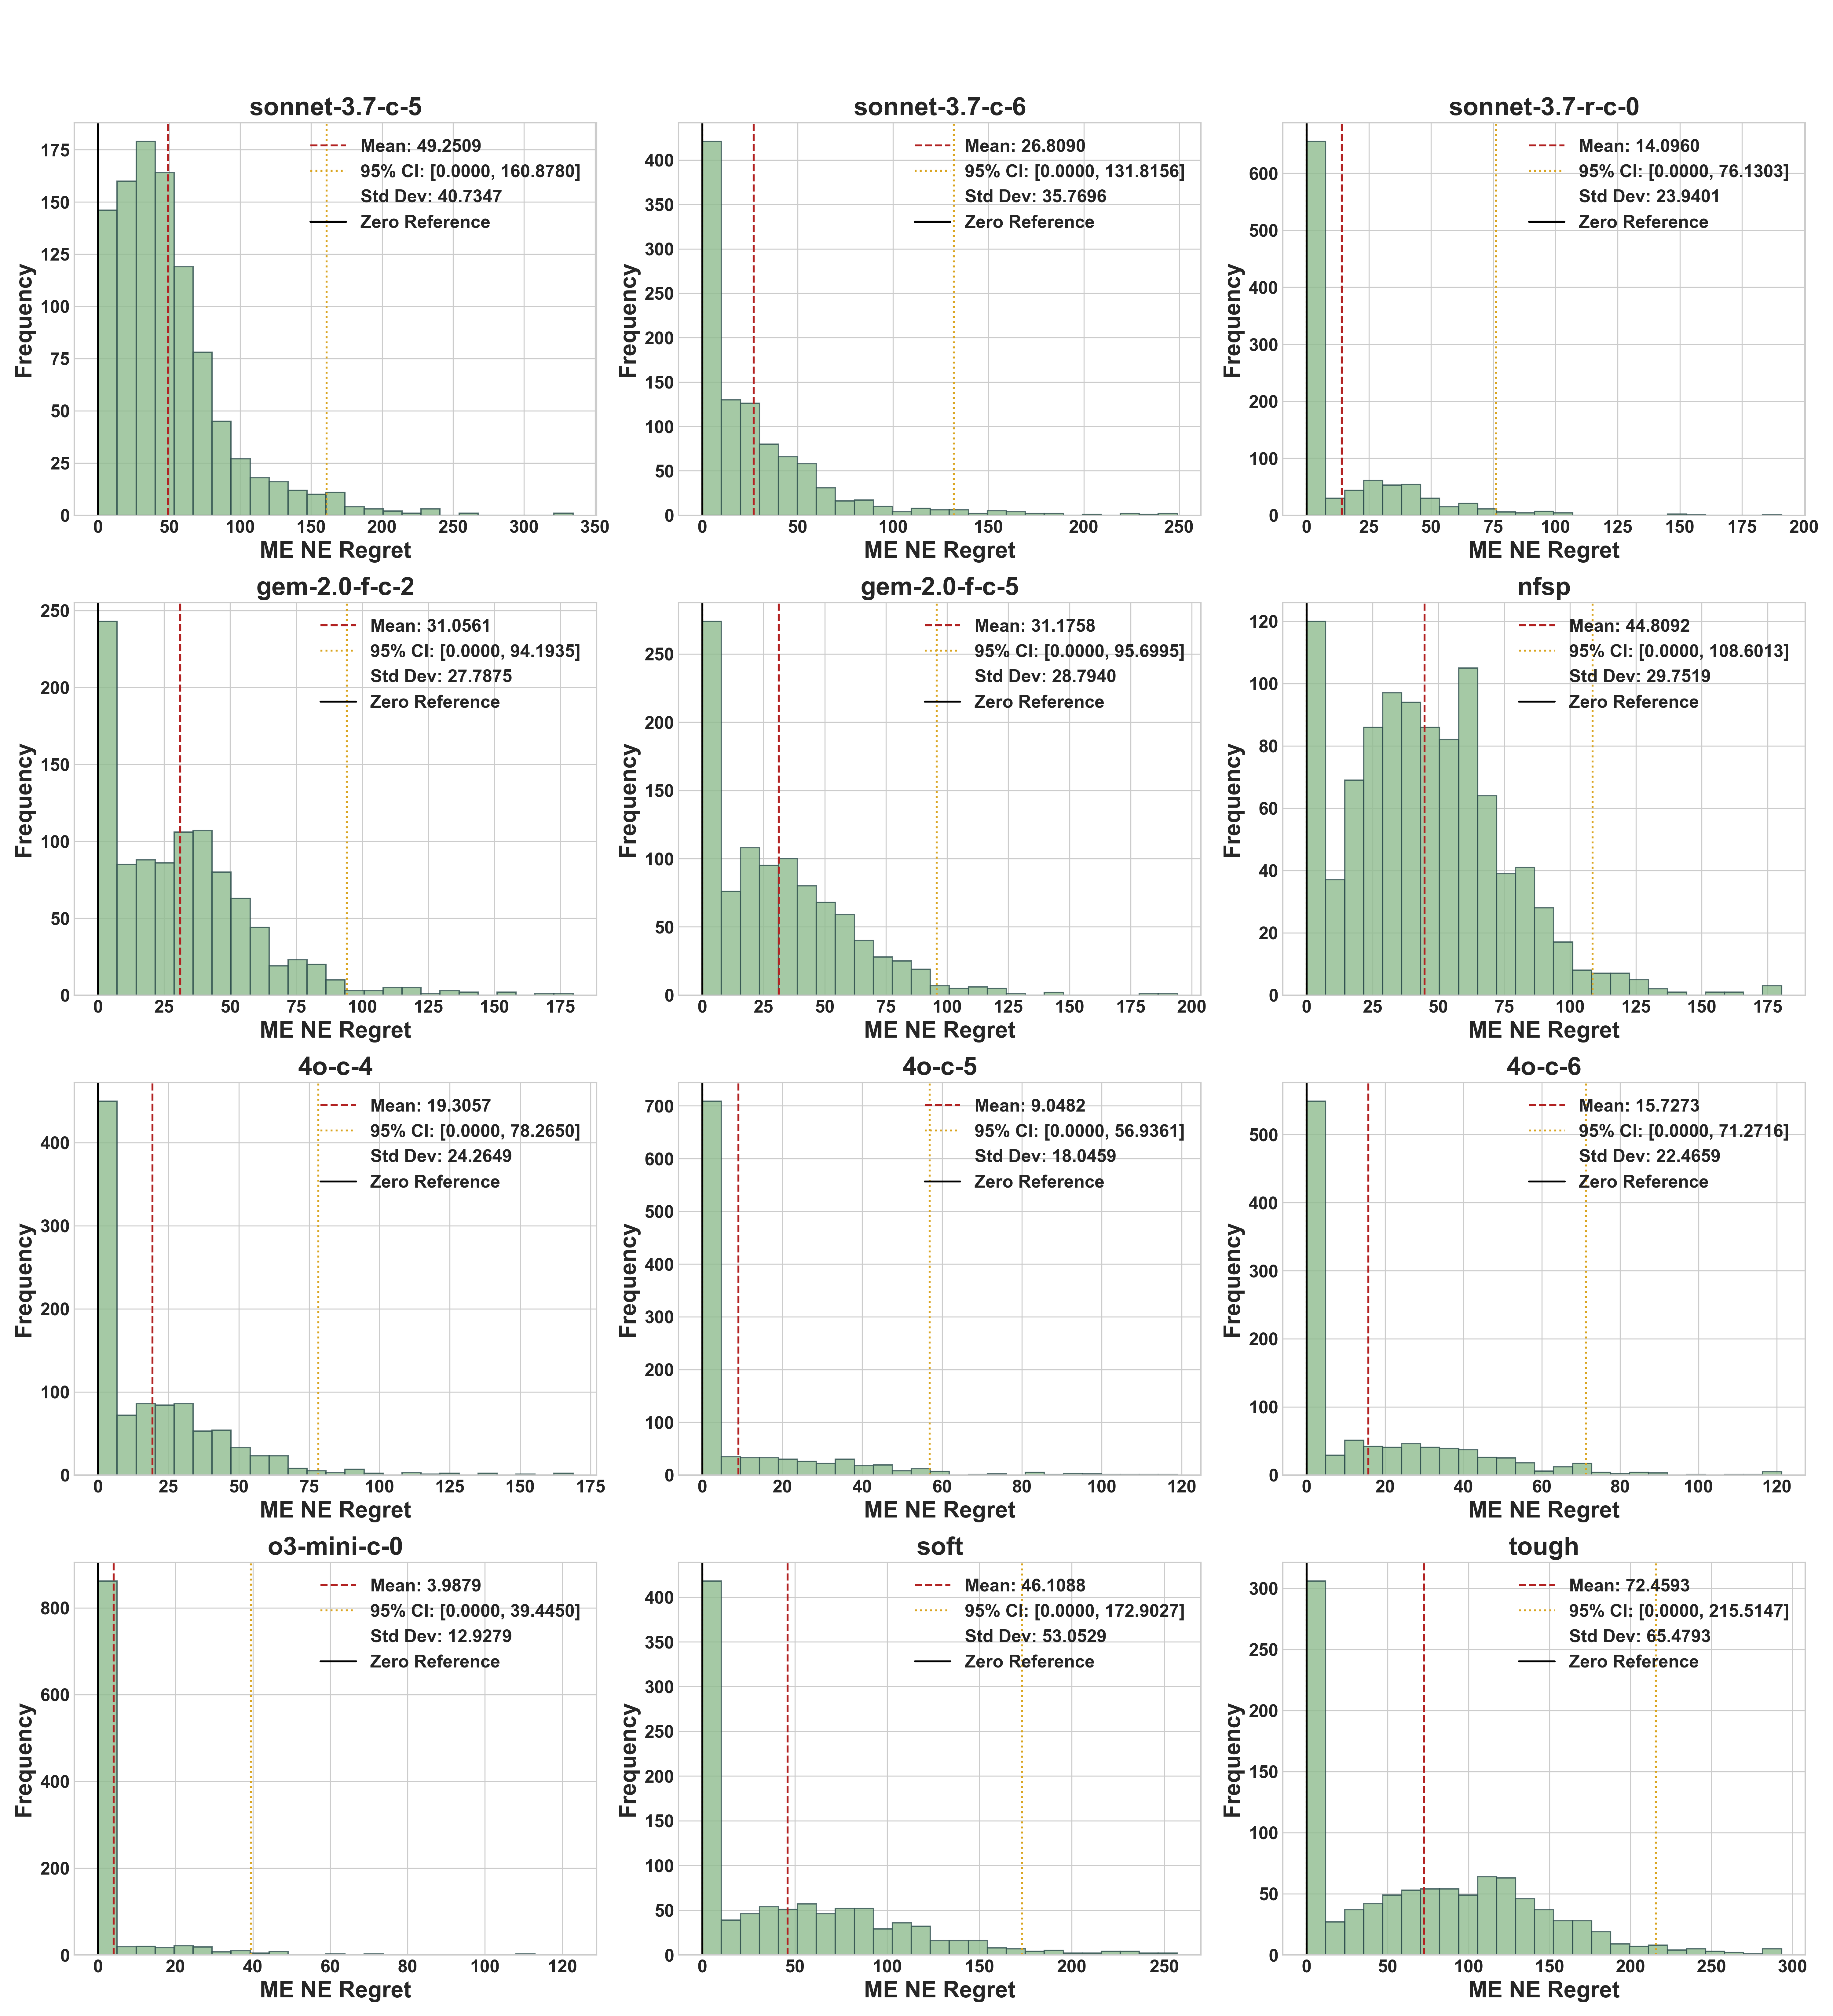
\includegraphics[width=0.46\textwidth]{icml_2025_workshop/bootstrap_distributions/LLM+NonLLM/game_matrix_2/me_ne_regret.png} &
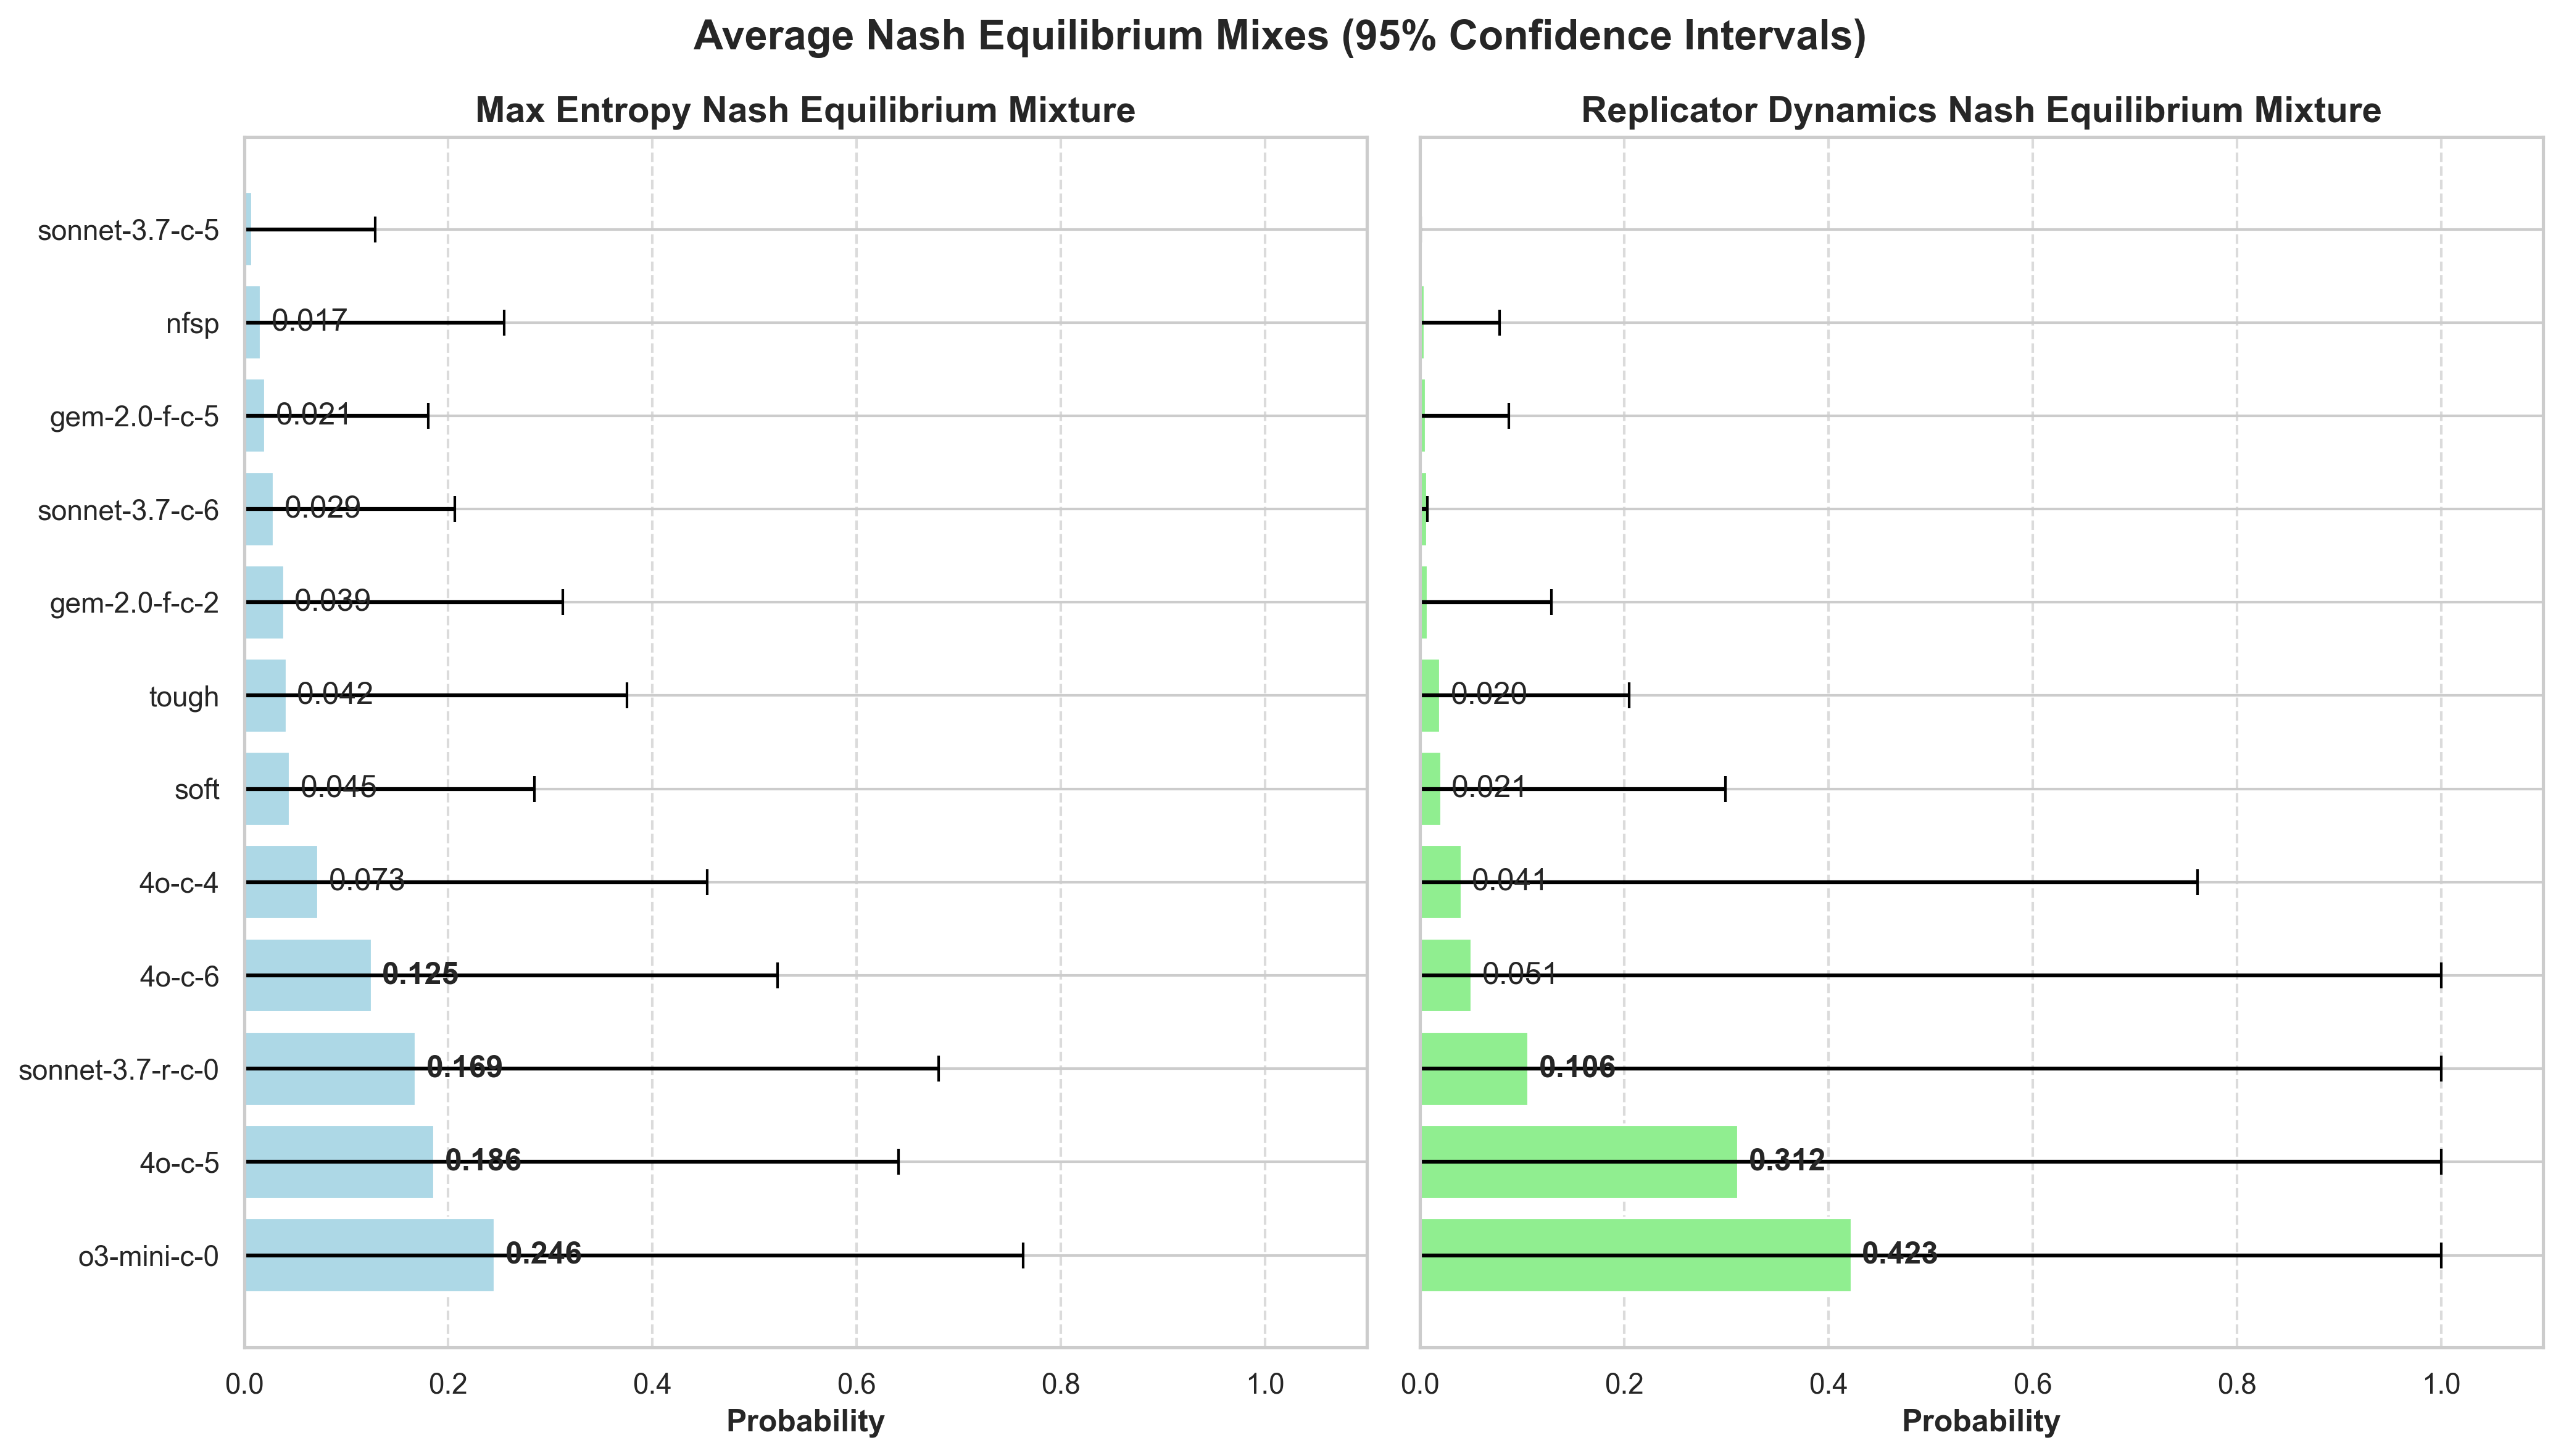
\includegraphics[width=0.46\textwidth]{icml_2025_workshop/bootstrap_distributions/LLM+NonLLM/game_matrix_2/nash_mixture.png} \\
{\small ME-NE Regret} & {\small Nash Mixture}
\end{tabular}
\caption{Mixed LLM/non-LLM bootstrap distributions for BG1 and BG2}
\label{fig:mixed_bg1_bg2}
\end{figure}

\vspace{0.5cm}

\begin{figure}[H]
\centering
\begin{tabular}{cc}
\multicolumn{2}{c}{\textbf{BG3 (\(\gamma=0.98\), \(R=5\))}} \\
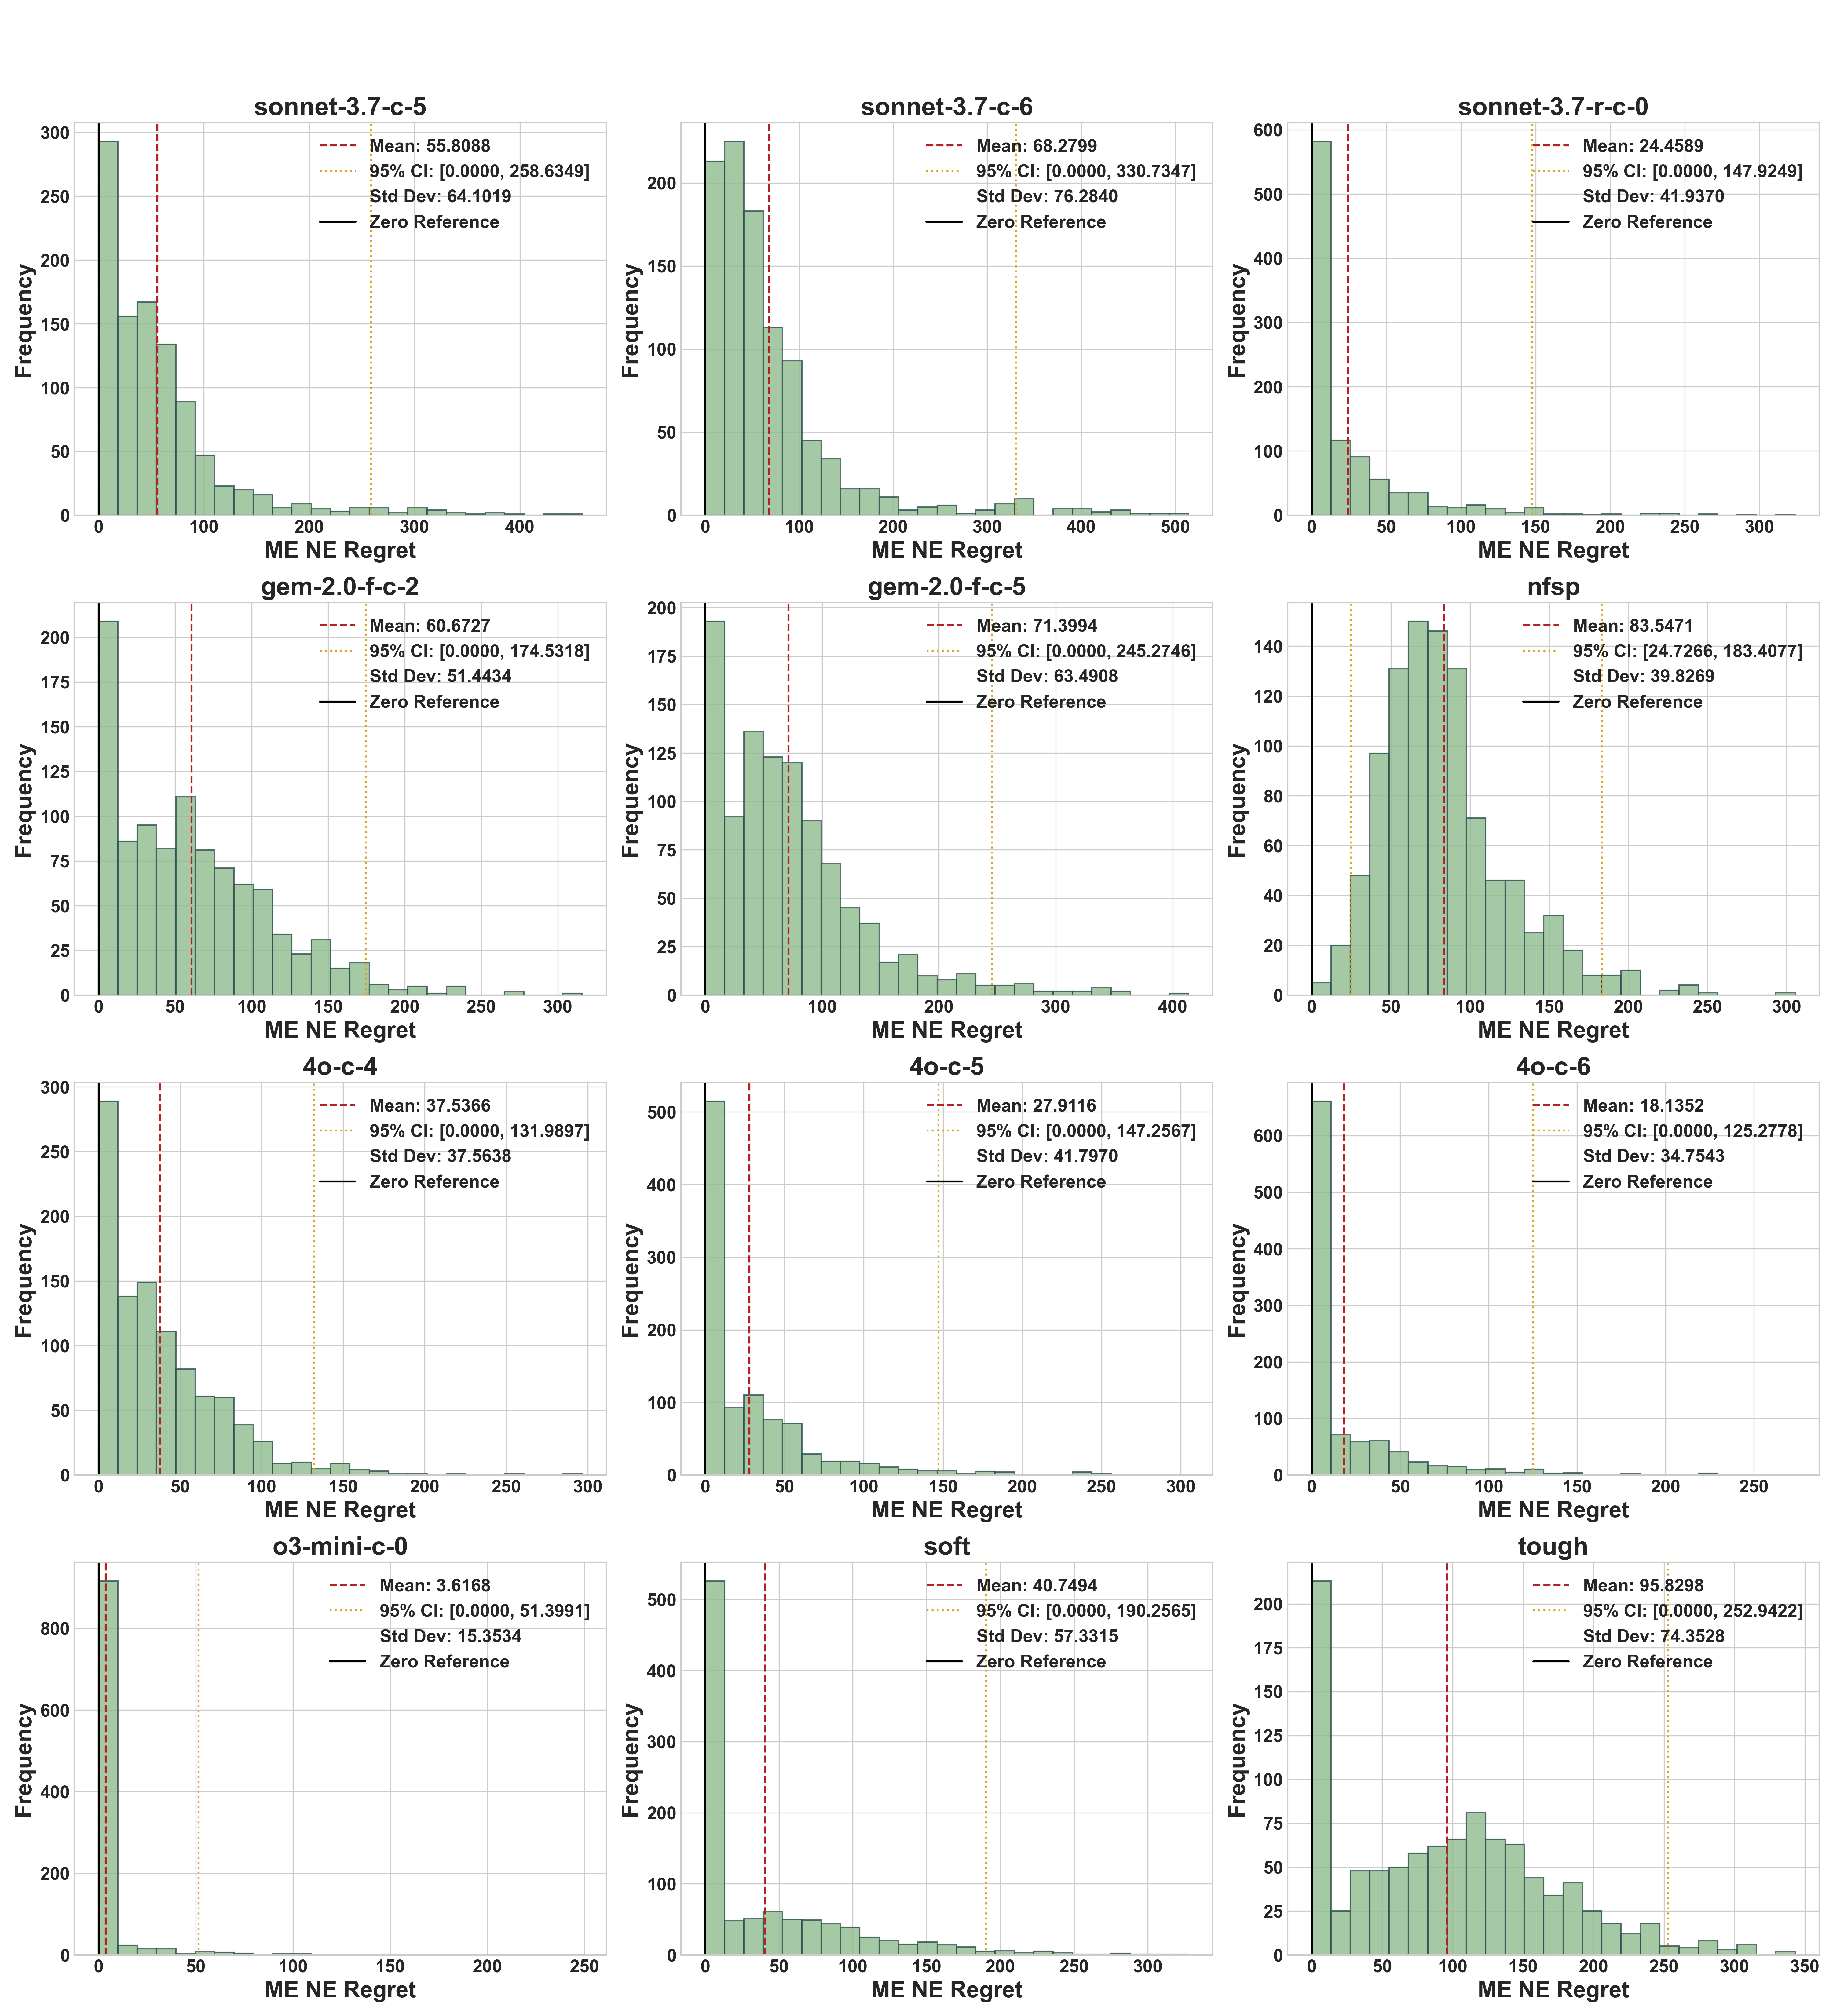
\includegraphics[width=0.46\textwidth]{icml_2025_workshop/bootstrap_distributions/LLM+NonLLM/game_matrix_3/me_ne_regret.png} &
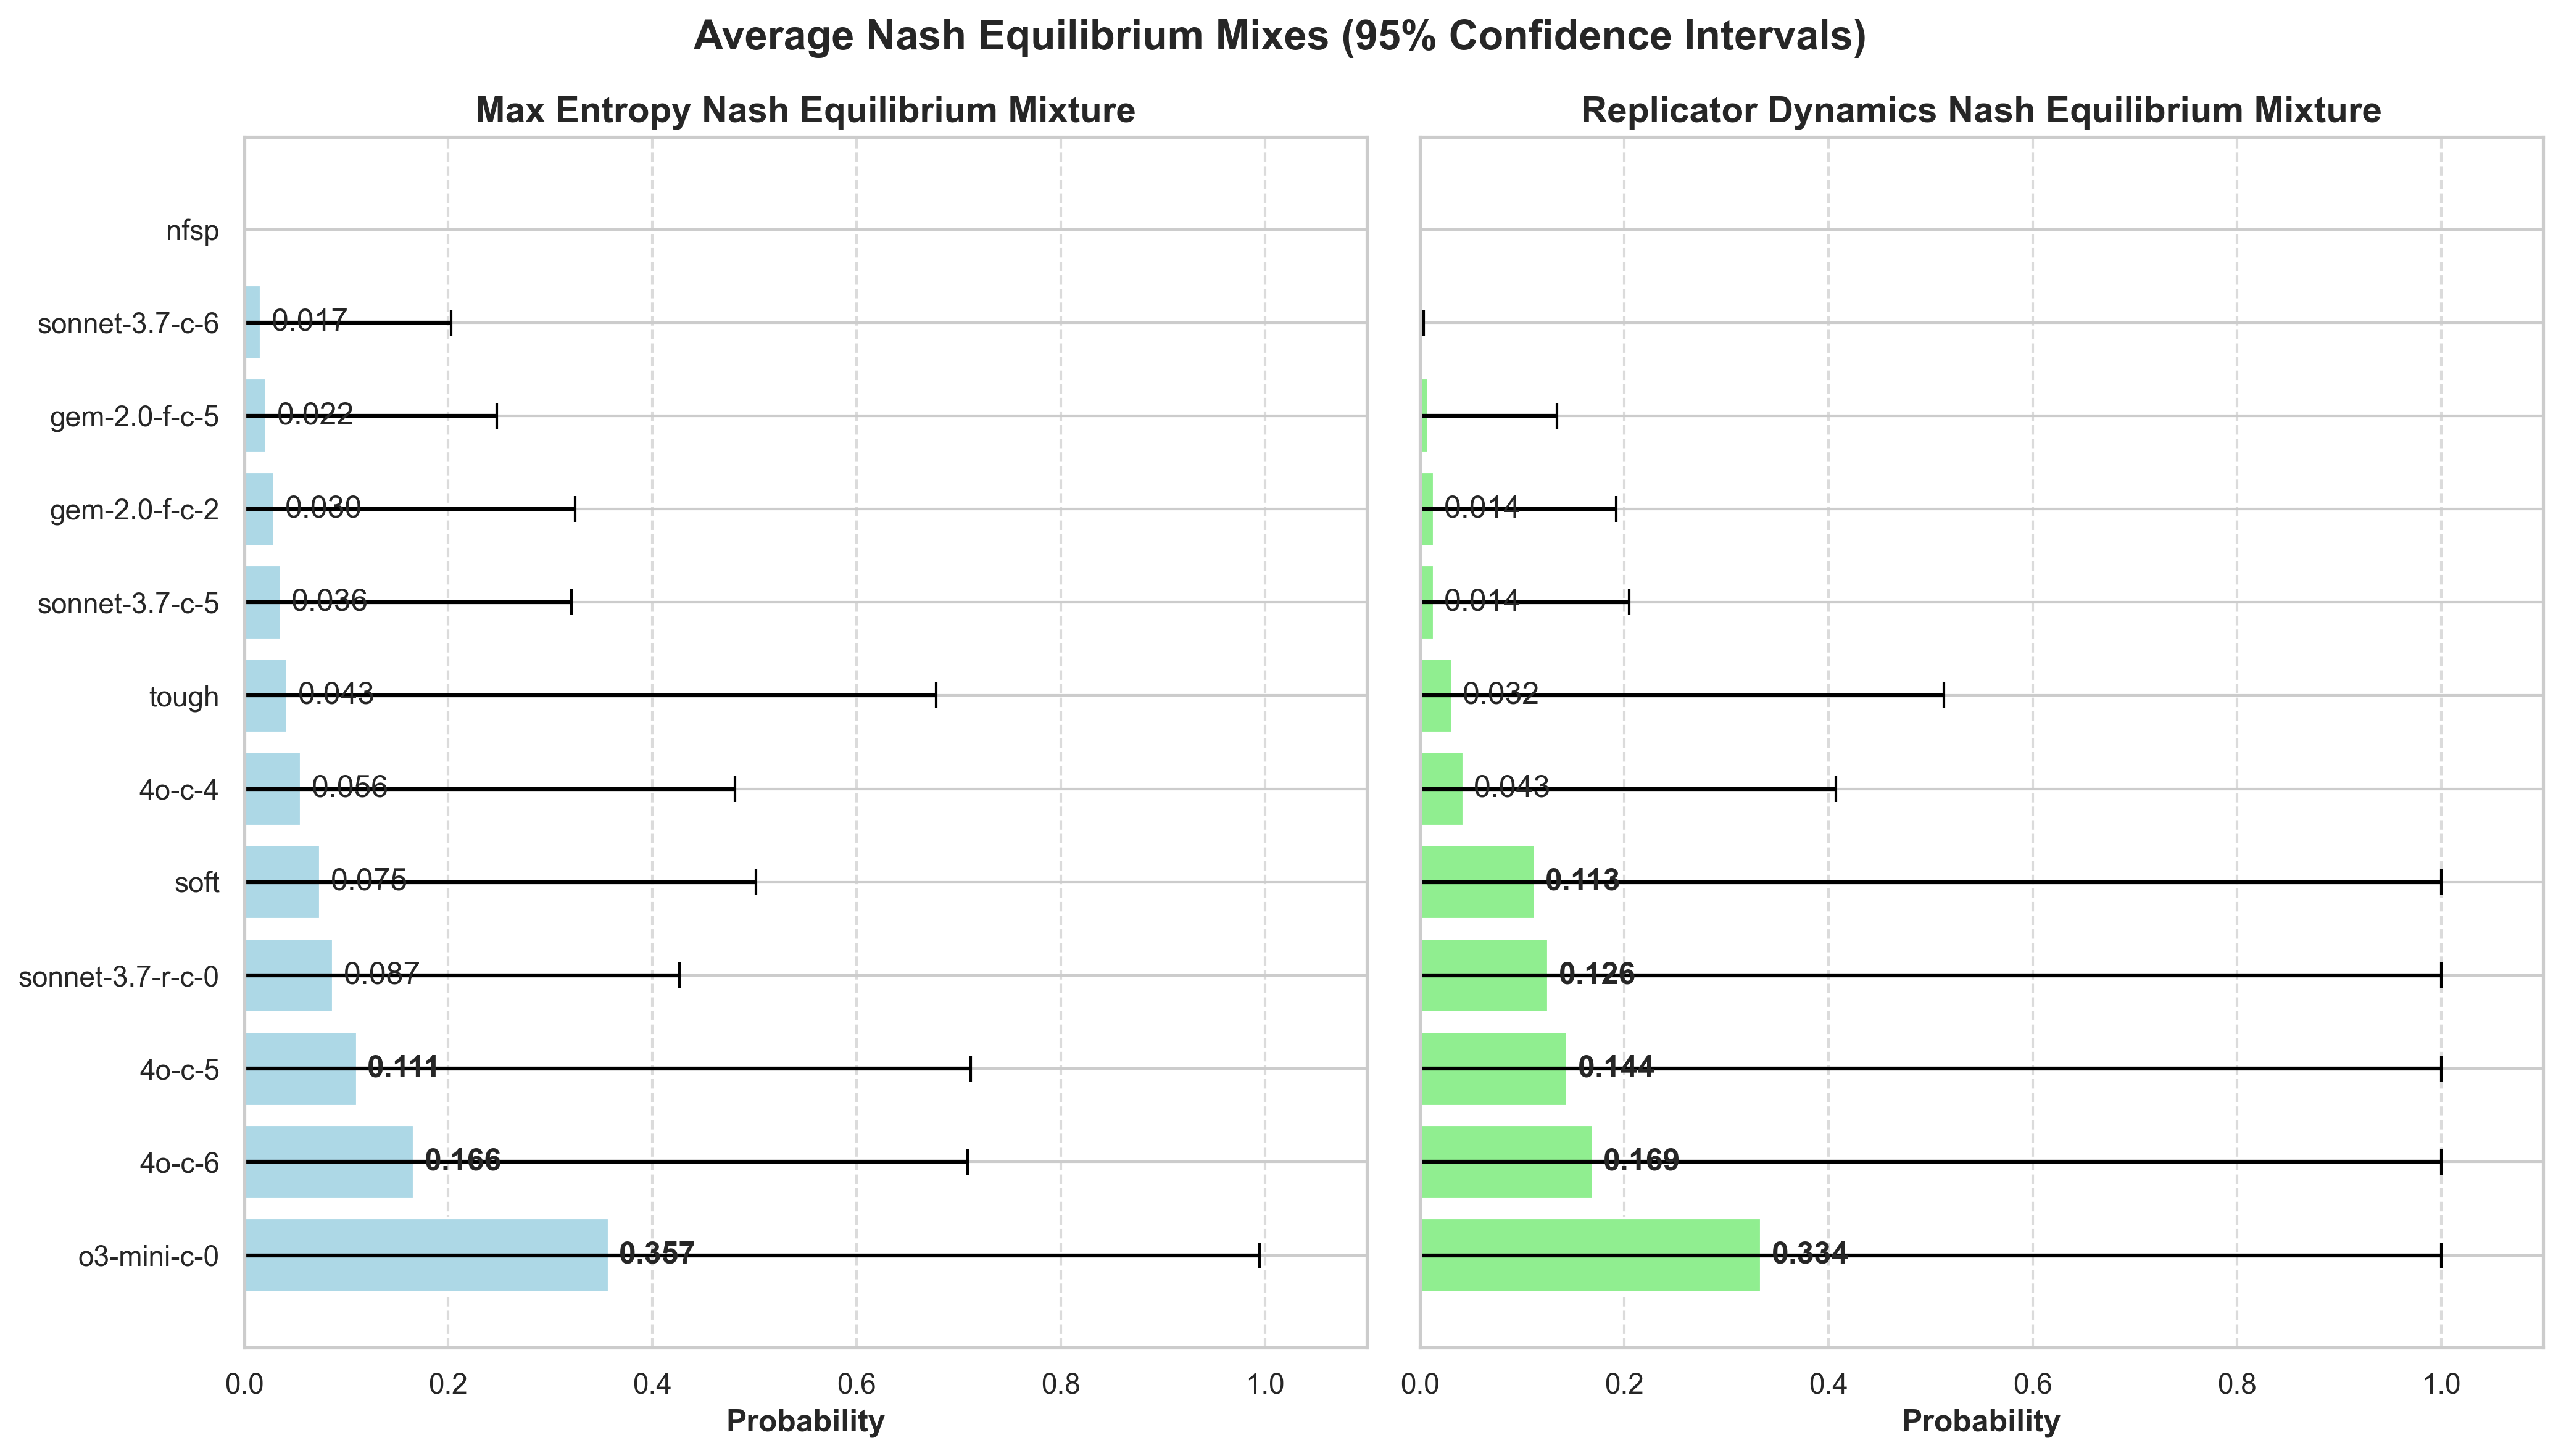
\includegraphics[width=0.46\textwidth]{icml_2025_workshop/bootstrap_distributions/LLM+NonLLM/game_matrix_3/nash_mixture.png} \\
{\small ME-NE Regret} & {\small Nash Mixture} \\%[0.5cm]

\multicolumn{2}{c}{\textbf{BG0 (meta-game over BG1-BG3)}} \\
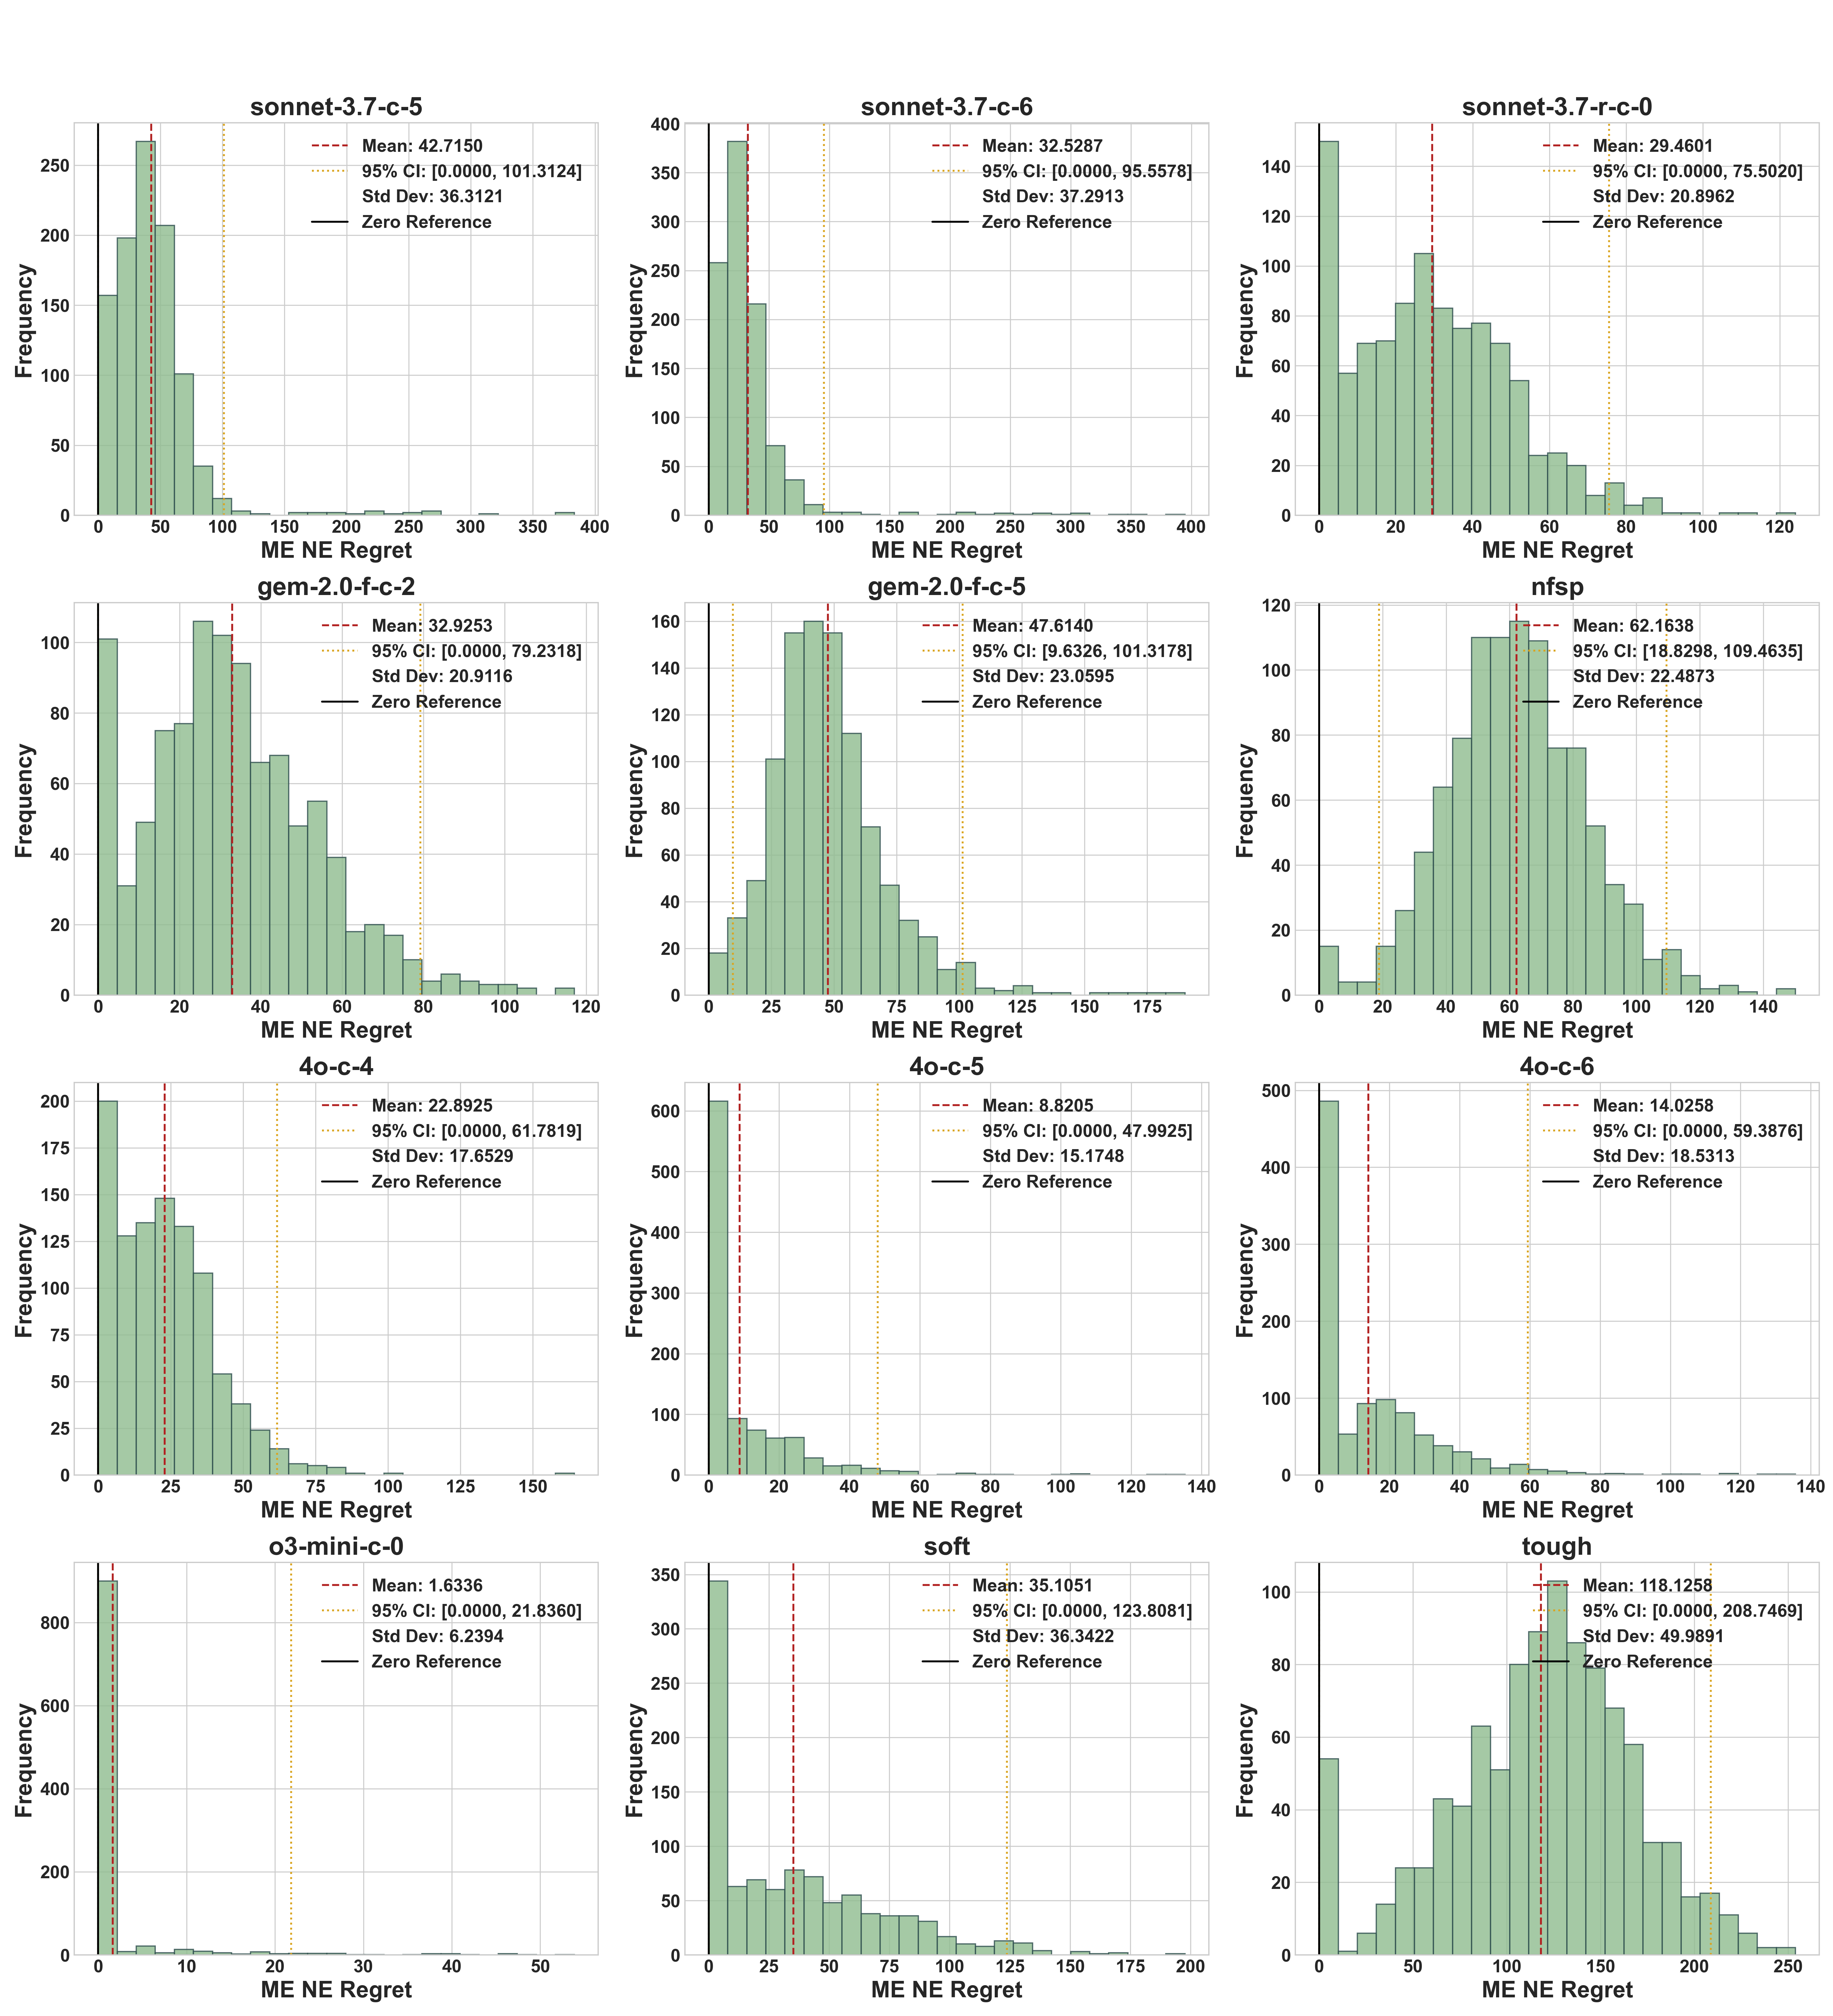
\includegraphics[width=0.46\textwidth]{icml_2025_workshop/bootstrap_distributions/LLM+NonLLM/game_matrix_4/me_ne_regret.png} &
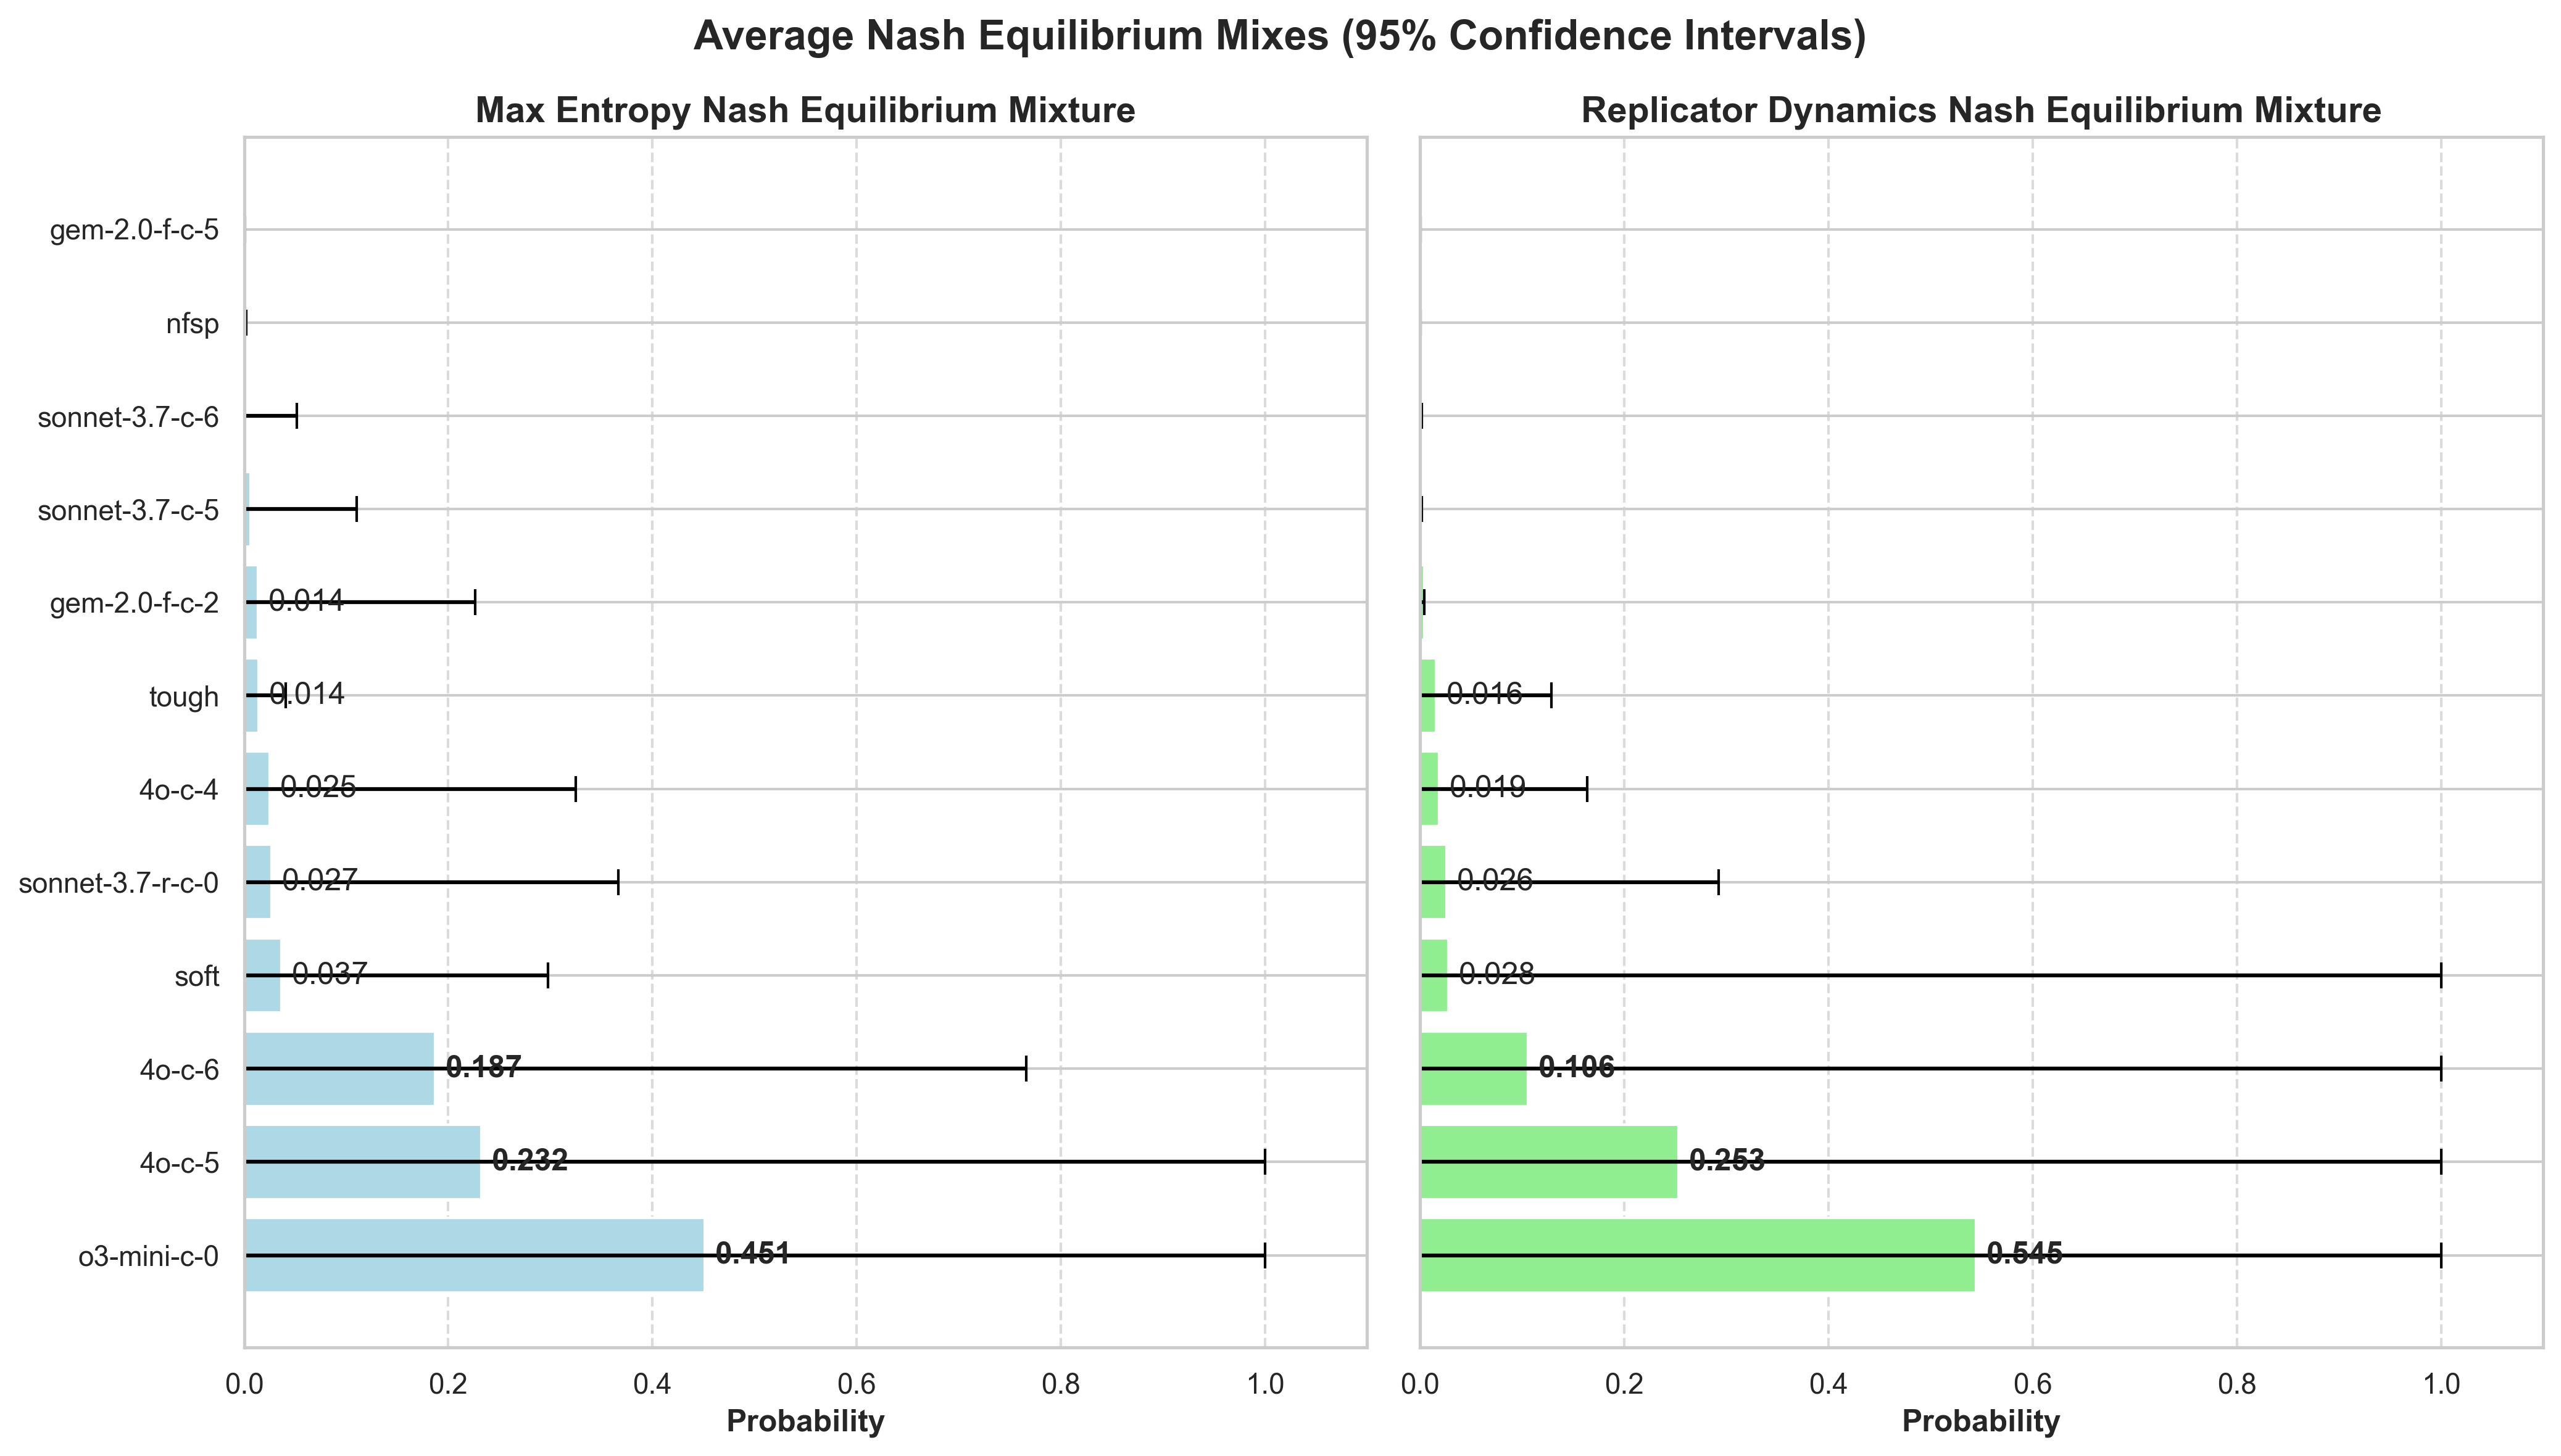
\includegraphics[width=0.46\textwidth]{icml_2025_workshop/bootstrap_distributions/LLM+NonLLM/game_matrix_4/nash_mixture.png} \\
{\small ME-NE Regret} & {\small Nash Mixture}
\end{tabular}
\caption{Mixed LLM/non-LLM bootstrap distributions for BG3 and BG0}
\label{fig:mixed_bg3_bg0}
\end{figure}

\section{Negotiation Mistakes}
\label{app:mistakes}

In any bargaining interaction, certain moves should be avoided to maintain rational play.  The five key mistakes, with illustrative examples, are:

\begin{enumerate}

  \item \textbf{Making an offer worse than your previous offer.}  
    You reject an opponent’s proposal that would have given you more value than the counteroffer you then make.  
    \\
    \textit{Example:} Suppose your private values per unit are $v=[4,2]$ for items A and B.  Your opponent offers you $(3,0)$, worth $3\cdot4 + 0\cdot2 = 12$. You then counter with $(2,0)$ (worth $8$), you have made a strictly worse proposal than the one you just rejected.

  \item \textbf{Making an offer worse for you than your outside offer.}  
    You propose a split in which the items you keep are worth less than your guaranteed fallback (outside offer).  
    \\
    \textit{Example:} Your outside‐offer value is $10$.  You propose to keep $(1,1)$, worth $1\cdot4 + 1\cdot2 = 6$, even though walking away would guarantee you $10$. 

  \item \textbf{Offering no items or all items.}  
    Issuing an extreme division—giving everything away or keeping everything.  
    \\
    \textit{Example:} In Round 2 of a 5‐round game, you offer to give the opponent all items $(0,0)$ for yourself. 

  \item \textbf{Accepting an offer worse for you than your outside offer.}  
    You agree to a deal that yields you less value than you would have secured by walking away to your outside option.  
    \\
    \textit{Example:} Your outside‐offer value is $8$.  Your opponent offers you $(1,0)$, worth $4$.  If you accept, you receive $4<8$, which is dominated by simply walking away.

  \item \textbf{Walking away from an offer better than your outside offer.}  
    You reject a valid split that provides you more value than your fallback, thus foregoing a strictly superior outcome.  
    \\
    \textit{Example:} Your outside‐offer value is $9$.  The opponent offers you $(2,1)$, worth $2\cdot4 + 1\cdot2 = 10$.  Walking away would leave you with $9$, so walking away is strictly dominated by the current offer on the table. 
  
\end{enumerate}


\section{Prompt Circles Used for Negotiation Models}
\label{app:prompting}

This section describes each incremental "circle" of prompts provided to the negotiation models. Each circle adds guidance or strategic considerations aimed at progressively improving the reasoning and negotiation outcomes. The circles follow a progression, with each level introducing more sophisticated negotiation concepts.

The negotiation history is maintained throughout the game, displaying each player's actions chronologically. The current offer on the table is explicitly stated, and the action prompt varies based on whether the agent is Player 1 making the first move, has a current offer to consider, or needs to make a counteroffer.

\subsection{System Prompt}
All LLM agents receive a consistent system prompt that establishes their role as negotiators and enforces the required response format:

\begin{Verbatim}[breaklines,fontsize=\small]
You are an AI negotiator participating in a negotiation game.

You must respond in one of these formats ONLY:
1. {"action": "ACCEPT"}
2. {"action": "WALK"}
3. {"action": "COUNTEROFFER", "offer": [n1, n2, ...]}

Ensure your response is valid JSON and matches one of these exact formats.
\end{Verbatim}

This system prompt is sent with every API call across all models and prompt circles, ensuring consistent response formatting. The detailed game instructions and strategic guidance are provided in the user message, which varies according to the prompt circle level described below.

\subsection{Circle 0: The Vestibule (Setting The Stage)}
The baseline negotiation scenario provides the foundational rules of the negotiation game, including player identities, item quantities, private valuations, outside offers, and negotiation structure. No additional guidance is provided beyond the basic game mechanics.

\begin{Verbatim}[breaklines,fontsize=\small]
You and another agent have to negotiate a division of items between the two of you.
You are Player {my_player_num} and the other agent is Player {other_player_num}.
There are {T} types of items, called item 1 through item {T}.
There are {quantities} to divide.
Both you and Player {other_player_num} have a private value per unit of each item type.
These values are drawn from a uniform random distribution, ranging from 1 to {V-1}.
Your private values are {values}.
You have a private outside offer drawn from a uniform random distribution ranging from {p1_outside_offer[0]} to your total value of all items, which is {p1_outside_offer[1]}. Player {other_player_num} has a private outside offer drawn from a uniform random distribution ranging from 1 to their total value of all items.
Your outside offer value is {w}. 

The negotiation proceeds in {R} rounds.
There is a discount rate gamma = {g}, such that if the process concludes after r rounds the overall value of the negotiation to each player is their value for the outcome multiplied by gamma to the power (r-1).
At each round, Player 1 takes an action, followed by Player 2.
The possible actions are to ACCEPT the other player's current offer (if any), make a COUNTEROFFER, or WALK away. If the game gets to the last round, and player 2 chooses to make a counteroffer, this is treated as a WALK.
If a player chooses ACCEPT, the negotiation ends in a deal to divide the items according to the accepted offer.
The value of an outcome is determined by each player's private values per unit of each item and the quantities they receive in the deal. This value is adjusted by the discount factor, which is used to compute the present value of the negotiation outcome.
If a player chooses WALK, the negotiation ends without a deal, and each player receives the value of their private outside offer.
\end{Verbatim}

\subsection{Circle 1: The Limbo of Objectives}
Circle 1 explicitly introduces the negotiation objective, reminding the agent to maximize its negotiation outcome and to carefully consider its guaranteed alternative, the outside offer.

\begin{Verbatim}[breaklines,fontsize=\small]
[All instructions from Circle 0, plus:]
Your objective is to maximize your value of the outcome of the negotiation game. Remember, you have a guaranteed alternative: your outside offer.
\end{Verbatim}

\subsection{Circle 2: The Circle of Calculations}
Circle 2 provides concrete numerical examples illustrating how agents should evaluate potential counteroffers by explicitly calculating their total value, ensuring the counteroffers are superior to their outside offers.

\begin{Verbatim}[breaklines,fontsize=\small]
[All instructions from Circle 1, plus:]
Before making any counteroffer, you should calculate its total value to you and compare it to your outside offer value of {w}. 
For example, if you were considering offering the other player 2 units of each item (keeping 3 units of each for yourself), you would calculate:
3 units of item 1 = 3 × {values[0]} = {3*values[0]} (multiplying units by your value per unit)
3 units of item 2 = 3 × {values[1]} = {3*values[1]} (multiplying units by your value per unit)
3 units of item 3 = 3 × {values[2]} = {3*values[2]} (multiplying units by your value per unit)
3 units of item 4 = 3 × {values[3]} = {3*values[3]} (multiplying units by your value per unit)
3 units of item 5 = 3 × {values[4]} = {3*values[4]} (multiplying units by your value per unit)
Total value = {sum([3*values[i] for i in range(T)])} (sum of all item values)
\end{Verbatim}

\subsection{Circle 3: The Circle of Systematic Analysis}
Circle 3 introduces a systematic three-step questioning strategy designed to facilitate a comprehensive analysis:
\begin{enumerate}
\item Analysis of the current negotiation situation
\item Assessment of the value of current and potential offers
\item Decision-making based on comparative analyses
\end{enumerate}

\begin{Verbatim}[breaklines,fontsize=\small]
[All instructions from Circle 2, plus:]
The following step-by-step questions are designed to guide you through a comprehensive analysis. By systematically addressing these questions, you can evaluate the current state of the negotiation, assess potential offers, and make informed decisions. You must use the information that you acquired through the step-by-step questioning above to decide what action you will make.
Let's walk through this step by step:

1) First, analyze the current situation:
   - What is my outside offer value?
   - What are the values of the items involved?
   - What is the total pool of items?
   - How does the discount factor influence the value of accepting the current offer versus waiting for future offers?

2) Assess the value of offers:
   - For the current offer (if any): What is my total value if I accept it?
   - For potential counteroffers: What would be my total value for different proposed divisions?
   - How do these values compare to my outside offer value?

3) Make a decision based on the analysis:
   - Should I accept the current offer?
   - Should I walk away and take my outside offer?
   - Or should I propose a specific counteroffer?
\end{Verbatim}

\subsection{Circle 4: The Circle of Common Errors}
\label{mistakes}
Circle 4 identifies five common negotiation mistakes that conflict with the negotiation objectives:
\begin{itemize}
\item \textbf{Mistake 1:} Making an offer worse than your previous offer. This occurs when you reject an offer better for you than the one you subsequently propose.
\item \textbf{Mistake 2:} Making an offer worse for you than your outside offer. This happens if you propose giving away so much that what you keep is worth less than your guaranteed alternative.
\item \textbf{Mistake 3:} Offering no items or all items. Offering nothing (or everything) to the opponent (in the early or middle rounds) can be a clear suboptimal move.
\item \textbf{Mistake 4:} Accepting an offer worse for you than your outside offer. This occurs if you accept a division that yields a payoff lower than your guaranteed fallback.
\item \textbf{Mistake 5:} Walking away from an offer better than your outside offer. This occurs when you reject a division that actually yields a higher payoff than your fallback.
\end{itemize}

\begin{Verbatim}[breaklines,fontsize=\small]
[All instructions from Circle 3, plus:]
In the bargaining game, there are five mistakes you can make that conflict with your objectives. 
While these aren't the only possible errors, they represent undesirable negotiation behaviors that can undermine your payoff or cause you to miss out on better deals. 
These mistakes are:
- Mistake 1: Making an offer worse than your previous offer. This occurs when you reject an offer better for you than the one you subsequently propose. 
- Mistake 2: Making an offer worse for you than your outside offer. This happens if you propose giving away so much that what you keep is worth less than your guaranteed alternative, which is your outside offer.
- Mistake 3: Offering no items or all items. Offering nothing (or everything) to the opponent (in the early or middle rounds) can be a clear suboptimal move. 
- Mistake 4: Accepting an offer worse for you than your outside offer. This occurs if you accept a division that yields a payoff lower than your guaranteed fallback.
- Mistake 5: Walking away from an offer better than your outside offer. This occurs when you reject a division that actually yields a higher payoff than your fallback.
\end{Verbatim}

\subsection{Circle 5: The Circle of Error Prevention}
Circle 5 provides explicit examples and strategic recommendations to prevent the identified mistakes, emphasizing the calculation of offer values and iterating proposals until surpassing the outside offer value. The specific example is dynamically generated for each player in each  game instance. This circle introduces a concrete example of a suboptimal offer to illustrate the importance of value calculation.

\begin{Verbatim}[breaklines,fontsize=\small]
[All instructions from Circle 4, plus:]
To prevent these mistakes, adopt a strategy similar to the following example: Before making any counteroffer, 
calculate its total value to you and compare it to your outside offer value. For instance, suppose you keep only {example_offer_less_than_outside_offer_self} items and offer the rest to the other party. Your value would be:
{values[0]} x {example_offer_less_than_outside_offer_self[0]} + {values[1]} x {example_offer_less_than_outside_offer_self[1]} + {values[2]} x {example_offer_less_than_outside_offer_self[2]} + {values[3]} x {example_offer_less_than_outside_offer_self[3]} + {values[4]} x {example_offer_less_than_outside_offer_self[4]}
which is {np.dot(values, example_offer_less_than_outside_offer_self)} (sum of all item values)

which is less than your outside offer of {w}. If your proposed offer results in a value lower than your outside offer, continue iterating until you develop a more advantageous offer that is better than your outside offer. 
This reasoning can be applied to each of the five highlighted mistakes to ensure that your offers align with your objectives and avoid undesirable negotiation behaviors.
\end{Verbatim}

\subsection{Circle 6: The Circle of Strategic Inference}
Circle 6 introduces strategic inference about the opposing agent's valuations based on their negotiation behavior. Agents are guided to infer relative valuations from the distribution of items in the opponent's offers, leveraging this information to inform their own negotiation strategy.


\begin{Verbatim}[breaklines,fontsize=\small]
[All instructions from Circle 5, plus:]
Keep in mind the offers the opposing agent makes reflects its own values. If their offer includes most or all units of a particular item, it might indicate that the agent does not highly value that item, whereas offering none could suggest the opposite. 
You can use this kind of evidence to help inform your decision-making.
\end{Verbatim}

\subsection{Response Format and History Tracking}
All prompts include standardized action specification requirements and maintain negotiation history across rounds:

\begin{Verbatim}[breaklines,fontsize=\small]
Please show your reasoning step by step, then provide your action in one of these formats in your response (if you do not do this your response will be invalid):
{"action": "ACCEPT"} - to accept the current offer
{"action": "WALK"} - to walk away from negotiations  
{"action": "COUNTEROFFER", "offer": [n1, n2, ...]} - where n1, n2, ... are numbers representing the number of units of each item being offered to the other player as part of the counteroffer.

Any response not in these exact formats will be invalid and treated as a WALK. If you provide a counteroffer, it must be a valid offer, otherwise it will be treated as a WALK.

It is now round {r}.

Negotiation history:
[History of all previous rounds, including offers made and actions taken]

Current offer on the table (the amount of each item being offered to you): {current_offer}

What is your action? [Action prompt specific to the current game state]
\end{Verbatim}

\subsection{Circle Selection Methodology}
We determined the prompt circle for each model through empirical testing in self-play scenarios, tracking the frequency of mistakes (as defined in Section~\ref{mistakes}). We aimed to select the circles that minimized errors, though in some cases the choice was not straightforward. For example, with \texttt{Gemini-2.0-flash}, no single circle consistently outperformed the others, so we made on judgment call based on overall performance patterns.   Clear patterns emerged for some models (e.g., GPT-4o and Claude Sonnet 3.7 showed substantial improvement with higher circles), while others showed minimal sensitivity to prompt complexity (e.g., Gemini 2.0 Flash). Reasoning models (o3-mini and Claude 3.7 Sonnet Reasoning) performed best with Circle 0, suggesting that additional instruction may interfere with their inherent reasoning capabilities.

\begin{figure}[H]
  \centering
  % First row
  \begin{subfigure}[b]{0.45\textwidth}
    \centering
    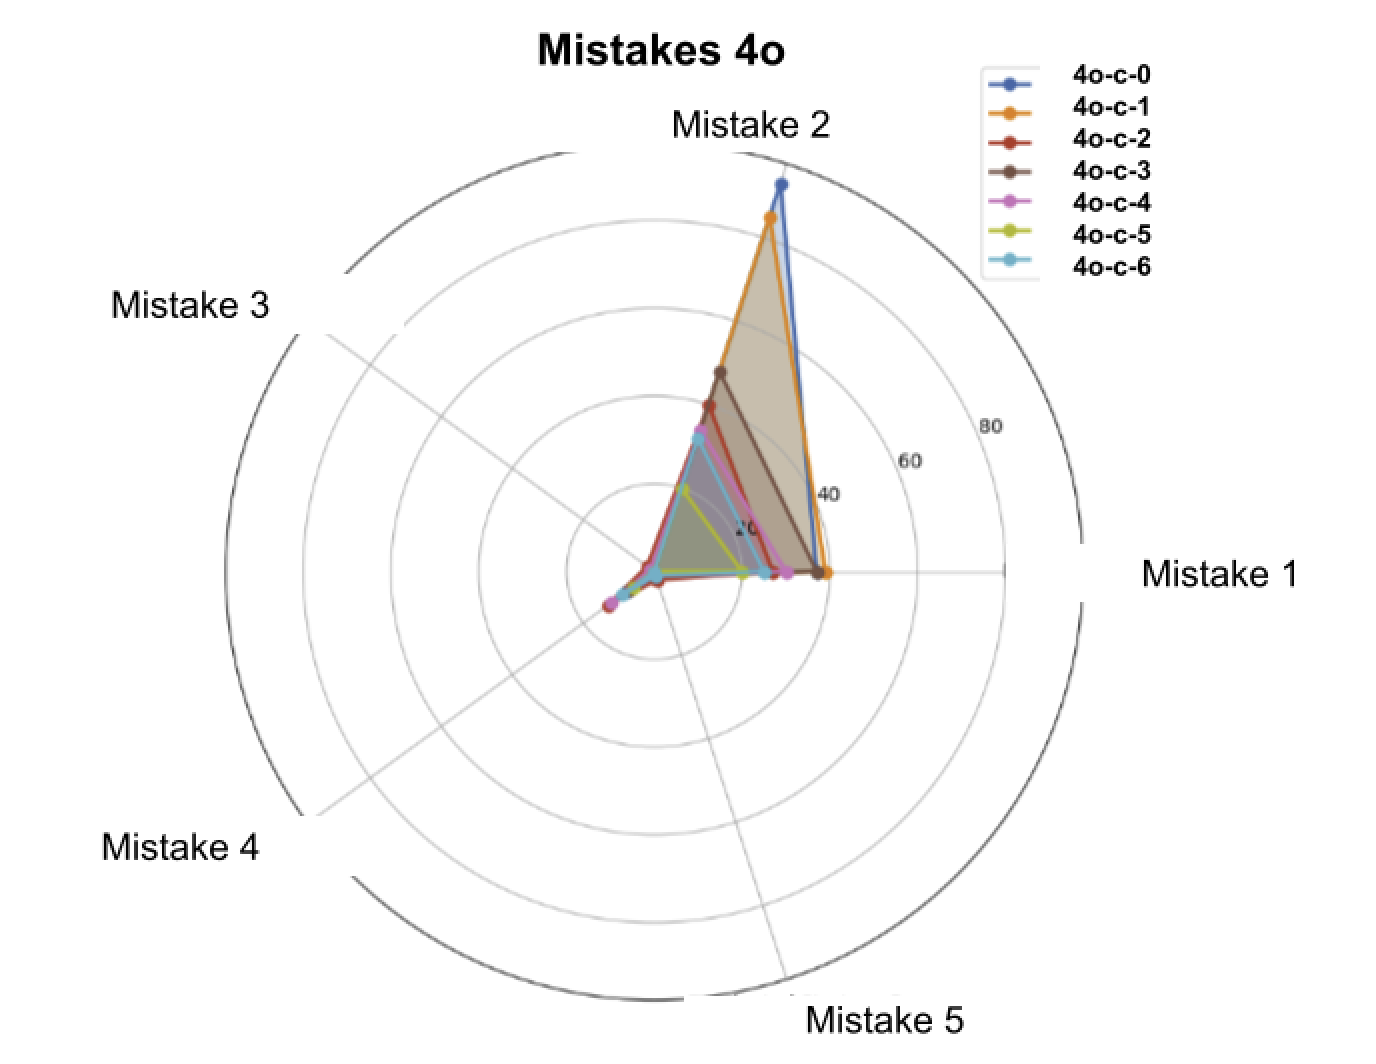
\includegraphics[width=\linewidth,height=\linewidth,keepaspectratio]{icml_2025_workshop/circles_dominiated_mistakes/4o_dominated_mistakes.png}
    \caption{GPT-4o: Number of mistakes per prompt circle.}
    \label{fig:4o-mistakes}
  \end{subfigure}
  \hfill
  \begin{subfigure}[b]{0.45\textwidth}
    \centering
    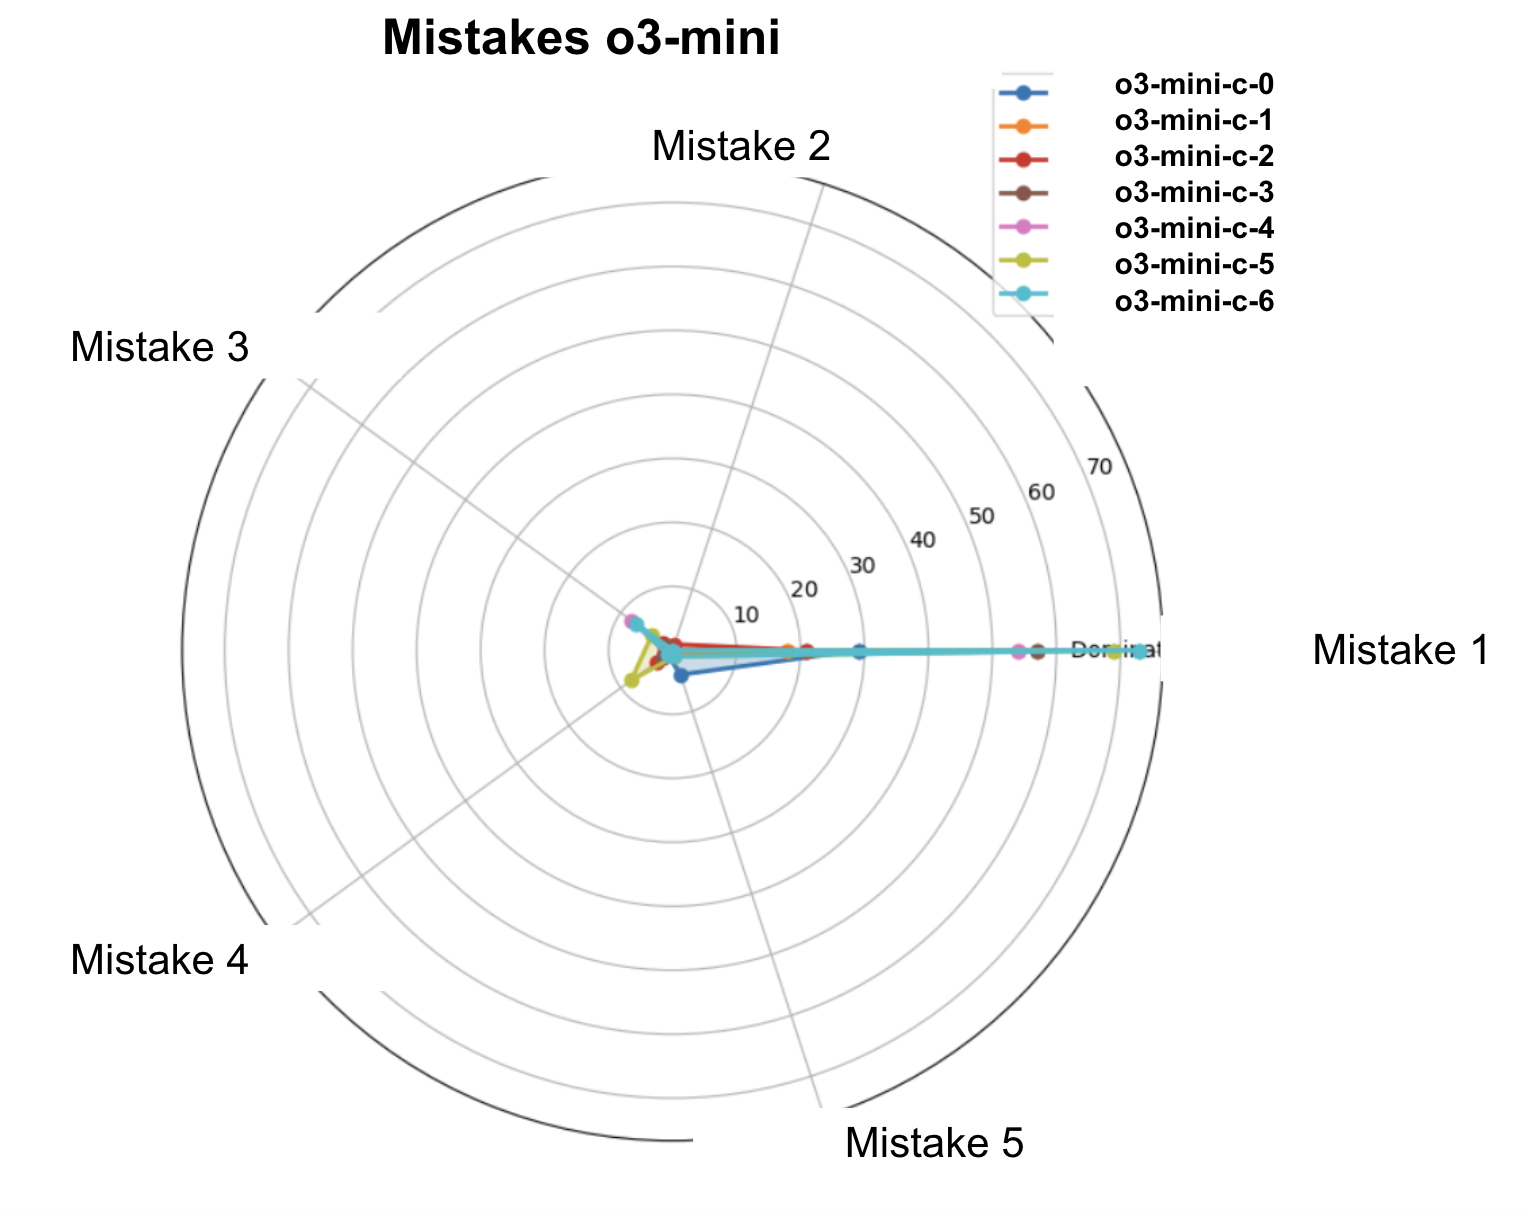
\includegraphics[width=\linewidth,height=\linewidth,keepaspectratio]{icml_2025_workshop/circles_dominiated_mistakes/o3_dominated_strategies.png}
    \caption{o3-mini: Impact of each prompt circle on strategy frequency.}
    \label{fig:o3-mistakes}
  \end{subfigure}

  \vspace{1em}

  % Second row
  \begin{subfigure}[b]{0.45\textwidth}
    \centering
    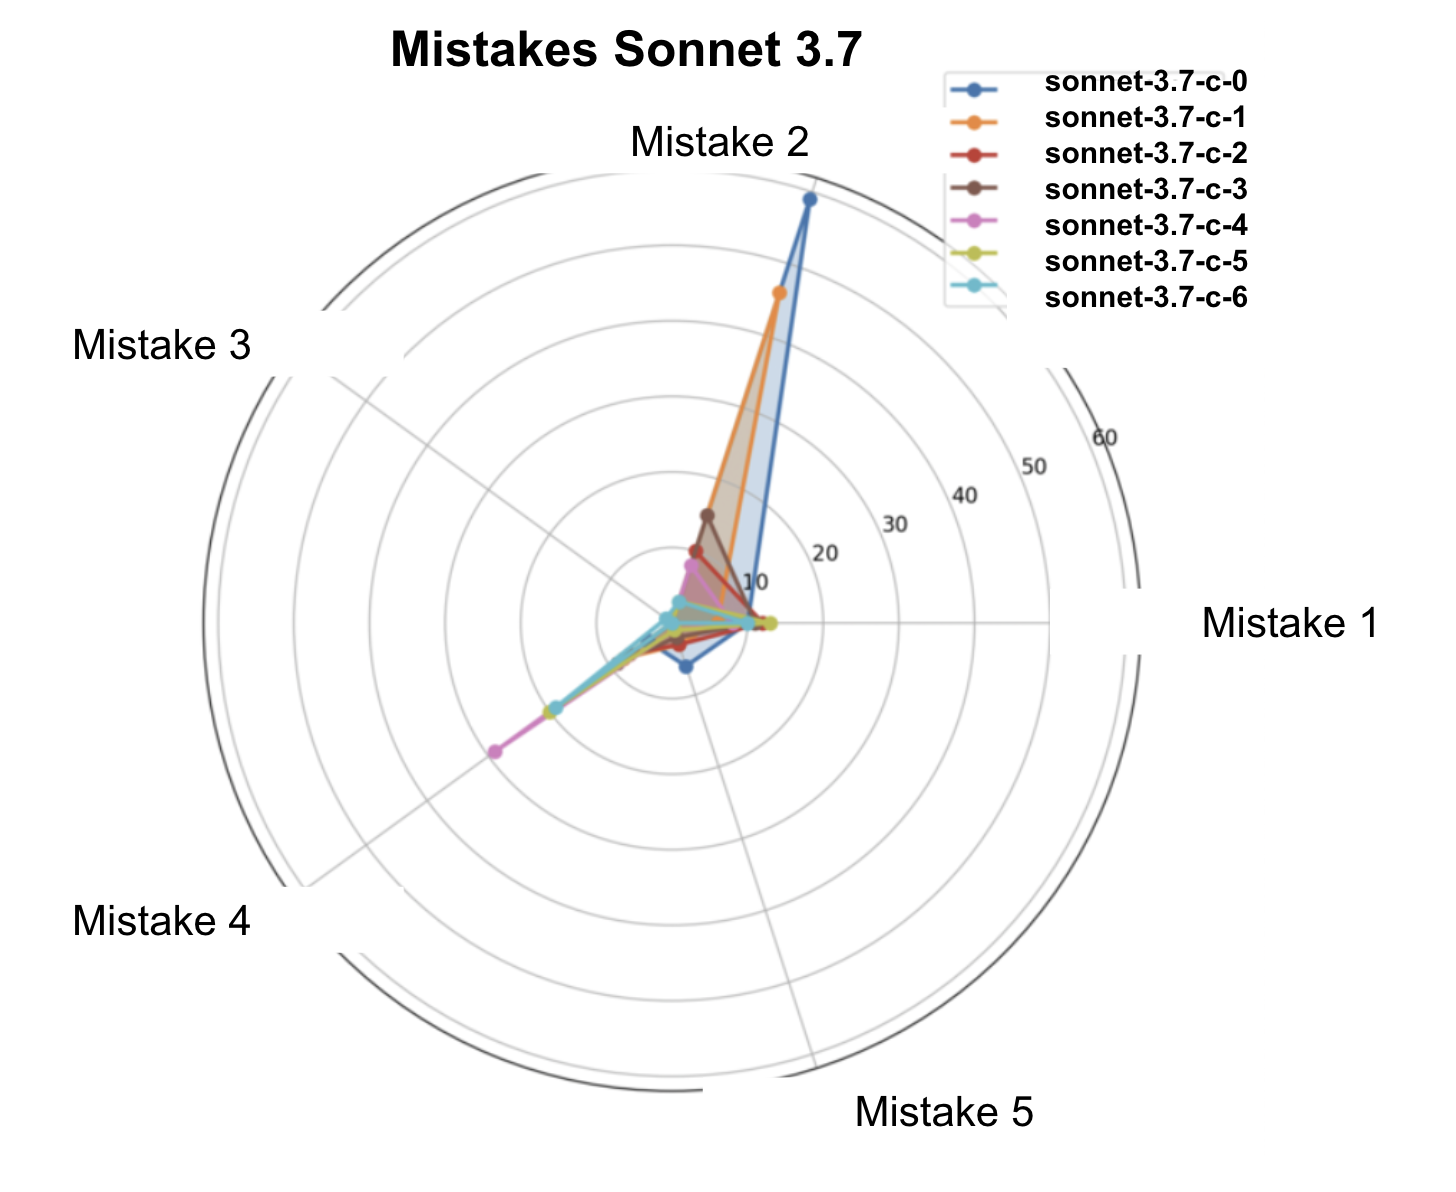
\includegraphics[width=\linewidth,height=\linewidth,keepaspectratio]{icml_2025_workshop/circles_dominiated_mistakes/sonnet_3.7_dominated_mistakes.png}
    \caption{Claude 3.7 Sonnet: Reduction in mistakes across circles.}
    \label{fig:sonnet-mistakes}
  \end{subfigure}
  \hfill
  \begin{subfigure}[b]{0.45\textwidth}
    \centering
    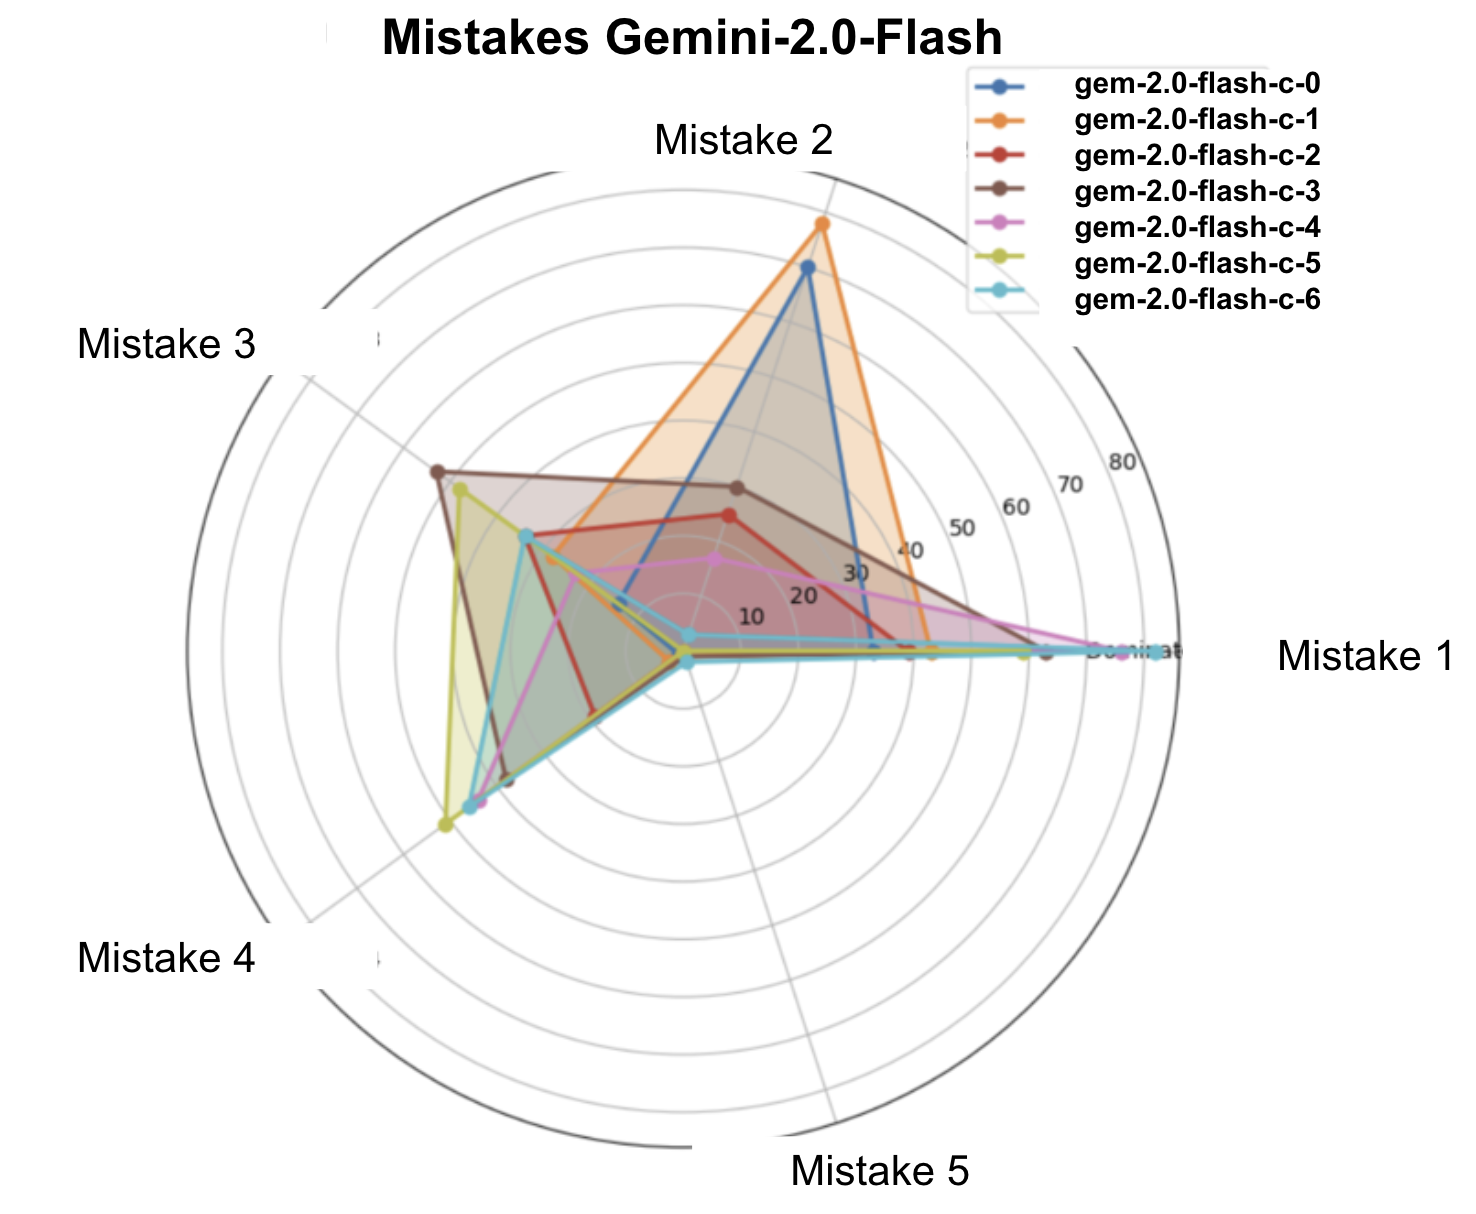
\includegraphics[width=\linewidth,height=\linewidth,keepaspectratio]{icml_2025_workshop/circles_dominiated_mistakes/gemini_flash_2.0_dominated_strategy.png}
    \caption{Gemini 2.0 Flash: Effectiveness of prompt circles on mistake avoidance.}
    \label{fig:gemini-mistakes}
  \end{subfigure}

  \caption[Mistakes by prompt circle across models]{\textbf{Mistake counts for each negotiation model as a function of prompt "circle."} Each subpanel shows the total number of mistakes (per Section~\ref{mistakes} definitions) made by that model under each incremental prompt circle (0–6). Lower bars indicate better adherence to rational negotiation behavior.}
  \label{fig:mistakes-by-circle}
\end{figure}


